

%%%%%%%%%%%%%% Document class
%%%\documentclass[a4paper,BCOR1.5cm,twoside,DIV12]{scrbook}
%\documentclass[a4paper,11pt,oneside,DIV15]{scrbook}
%\documentclass[a4paper,11pt,oneside,DIV15]{scrartcl}

% Sele��o do tipo de monografia e das op��es de formata��o
\documentclass[openright,diss]{deletex}

% um tipo espec�fico de monografia pode ser informado como par�metro opcional:
%\documentclass[tese]{deletex}

% O tipo de monografia pode ser:
% diss 			disserta��o de mestrado
% rp 			relat�rio de pesquisa
% prop-tese 		proposta de tese de doutorado
% plano-doutorado 	plano de curso de doutorado
% dipl-ele 		projeto de diploma��o em Engenharia El�trica
% dipl-ecp		projeto de diploca��o em Engenharia de Computa��o
% estagio		relat�rio de est�gio supervisionado 
% ti			trabalho individual
% pep			plano de estudos e pesquisa
% tese			tese de doutorado
% tc			trabalho de conclus�o de mestrado profissional
% espec			monografia de conclus�o de curso de especializa��o

% � importante notar que estes tipos de monografia foram herdados do estilo
% do II/UFRGS e n�o necessariamente aplicam-se ao DELET/EE/UFRGS. Ou seja,
% embora a classe deletex.cls defina uma opcao para elaborar um PEP, isto nao
% significa que um PEP seja exigido pelo PPGEE.

% monografias em ingl�s devem receber o par�metro `english':
%\documentclass[diss,english]{deletex}

% a op��o `openright' pode ser usada para for�ar in�cios de cap�tulos
% em p�ginas �mpares
% \documentclass[openright]{deletex}

% para gerar uma vers�o somente-frente, basta utilizar a op��o `oneside':
% \documentclass[oneside]{deletex}

% A opcao numbers pode ser usada para gerar refer�ncia num�ricas.
% A opcao sort&compress faz com que referencias do tipo [8,5,3,4] sejam
% convertidas para [3-4,8]
%\documentclass[numbers,sort&compress]{deletex}

% A opcao relnum faz com que a numeracao de figuras, tabelas e equa��es
% seja por cap�tulo.
%\documentclass[relnum]{deletex}


%%%%%%%%%%%%%%%%%%%%%%%%%%%%%%%%%%%%%%%%%%%%%%%%%%%%%%%%%%%%%%%%%%%%%%%%%%%%%%%%%%%%%%%%%%%%%%%%%%%%%%%%
% Preambule
\usepackage[latin1]{inputenc}   % Zeichensatz
\usepackage{graphicx}           % Einbinden von Grafiken
\usepackage{verbatim}
\usepackage{alltt}              % Verbatim-Umgebung mit Steuerbefehlen (z.B. fett, kursiv, ...)
\usepackage{booktabs}           % Paket f�r sch�nere Tabellen
\usepackage{subfigure}
\usepackage{url}
\usepackage{ae}
\usepackage{float}
\usepackage{psfrag}
\usepackage{amsfonts}
\usepackage{amssymb}
\usepackage{amsmath}
\usepackage{pstricks,pst-node,pst-text,pst-3d}
%\usepackage{hyperref}   % use for hypertext links, including those to external documents and URLs
%\usepackage[breaklinks=true]{hyperref}
%\usepackage[brazil]{babel} %get everything translated properly
\usepackage[brazilian]{babel} %get everything translated properly
%\selectlanguage{brazil}
%\usepackage[numbers]{natbib}
\usepackage{enumerate}
%\usepackage{newclude}

\usepackage{listings}           % Paket, um Listings sch�n einbinden zu k�nnen
\lstloadlanguages{Matlab}
%\usepackage[usenames,dvipsnames]{color}
%\usepackage{thumbpdf}           % Thumbnails f�r Seitenvorschau
%\usepackage{algorithm}
%\usepackage{algorithmicx}
%\usepackage{algpseudocode}
%\usepackage[portuguese,onelanguage,ruled,noline,linesnumbered]{algorithm2e}
%\usepackage[portuguese,ruled,noline]{algorithm2e}

%\usepackage{amsmath}
\usepackage{amsthm}
%\usepackage{amsfonts}
%\usepackage{amssymb}
%\usepackage{thmtools}
%\declaretheoremstyle[,
%bodyfont=\normalfont
%]{mystyle}
%\declaretheorem[name=Exemplo,style=mystyle,numberwithin=chapter]{example}
%\declaretheorem[name=Exemplo,numberwithin=section]{example}
%\usepackage{balance}
%\usepackage{setspace}
%
%\usepackage{multirow}
%\usepackage{rotating}
%
%\usepackage{subfig}
%\usepackage{fancyhdr}
%\usepackage{layout}
%\usepackage{chngpage}
%\usepackage{colortbl}
%\usepackage{float}
%\usepackage[intoc,noprefix]{nomencl}
\usepackage{tikz}
\usetikzlibrary{shapes,arrows}

%%\renewcommand{\nomname}{List of Symbols}

%\makenomenclature

%\usepackage{losymbol}

%%%\usepackage{makeidx}            % F�r Benutzung des Befehls \printindex
%%%\usepackage{flafter}            % Platziert Gleitobjekte nach ihrer Definition

%%%\usepackage{german}            % Erm�glich die direkte Eingabe von Umlauten
%%%\usepackage{bibgerm}           % Bitex: Deutscher Style der Literaturreferenzen
%\usepackage{caption}           % �berschriften f�r floating Umgebungen, %%z.B. f�r Tabellen und Bilder
%%%\usepackage{pslatex,times}     % Setzt die Schriftart Times als Standardschriftart
%%%\usepackage{nomencl}           % Legt eine Liste aller Symboldefinitionen (z.B. �P = ...) an
%%%\usepackage{textcomp}          % Zus�tzliche mathematische Symbole
%%%\usepackage{amssymb}           % Americam mathematican Society -> Symbole


%\usepackage{amsfonts}% to get the \mathbb alphabet
%\newcommand{\field}[1]{\mathbb{#1}}
%\newcommand{\setc}[1]{\mathcal{#1}}
%\newcommand{\C}{\field{C}}
%\newcommand{\R}{\field{R}}
%\newcommand{\vect}{\mathbf}
%\newcommand{\matr}{\mathbf}
%\renewcommand\Re{\operatorname{Re}}
%\renewcommand\Im{\operatorname{Im}}
%\newcommand{\pderfrac}[2]{\frac{\partial#1}{\partial#2}}
%\providecommand{\trans}[1]{{#1}^\mathrm{T}}

%\hhhypersetup{
%	colorlinks,
%	debug=true,
%	linkcolor=black,  %%% cor do tableofcontents, \ref, \footnote, etc
%	citecolor=red,  %%% cor do \cite
%	urlcolor=blue,   %%% cor do \url e \href
%	bookmarksopen=true,
%	pdftitle={Disserta��o de Mestrado},
%	pdfauthor={Tassiano Neuhaus},
%	pdfsubject={Projeto de controladores n�o lineares representados por modelos NARMAX usando refer�ncia virtual.},
%	pdfkeywords={System identification, data-base control design, Virttual Reference, nonlinear systems, NARMAX models},
%	%pdfpagemode=FullScreen
%}

%%%%%%%%%%%%%%%%%%%%%%%%%%%%%%%%%%%%%%%%%%%%%%%%%%%%%%%%%%%%%%%%%%%%%%%%%%%%%%%%%%%%%%%%%%%%%%%%%%%%%%%%%

% Setings for Code Listing
\lstset{
	language=VHDL,
	frame=single,
	commentstyle=\footnotesize,
	basicstyle=\footnotesize\ttfamily,
	%basicstyle=\small\ttfamily,%
	tabsize=1,%
	keywordstyle=\color{blue}\bfseries,%
	captionpos=b,  % caption position: bottom
	showstringspaces=false,
	numbers=left,%
	numberstyle=\footnotesize,
	%stepnumber=2,               % Abstand zwischen den Zeilennummern
	numbersep=1pt,              % Abstand der Nummern zum Text
	framexleftmargin=6mm,
	framexrightmargin=-6mm,%
	xleftmargin=6mm,
	xrightmargin=10mm,
	breaklines=true
	escapechar=$
}

\usepackage{pdflscape}

\usepackage{geometry}
\geometry{hcentering}
%%\geometry{a4paper,textwidth=153mm,textheight=224mm,top=35mm,hcentering}

%%%% Some self made macros


%%%%%%%%%%%%%%%%%%%%%%%%%%%%
%-+
%+ \TODO[<wer>]{<text>}
%+-
%- Erzeugt am Seitenrand den <text> mit dem zus�tzlichen
%- Vermerk, f�r <wen> dieses TODO noch offen ist.
%-
\newcommand{\TODO}[2][ICH]{%
\marginpar{\footnotesize \color{red} TODO [#1]:\\%
#2}}

%%%%%%%%%%%%%%%%%%%%%%%%%%%%
%
% \todobf{text}
%
\newcommand{\todobf}[1]{{\color{red}\textbf{TODO:  #1}}}


%%%%%%%%%%%%%%%%%%%%%%%%%%%%
%
% \note{text}
%
\newcommand{\note}[1]{{\color{red}\rule{0.5em}{1ex} \textbf{#1}}}

%%%%%%%%%%%%%%%%%%%%%%%%%%%%
%
% \tred{text}
%
\newcommand{\tred}[1]{{\textcolor{red}{#1}}}

%%%%%%%%%%%%%%%%%%%%%%%%%%%%
%
% Change the standard name "Bibliography" to "References", which is required by ABNT
%
\renewcommand\bibname{References}



%\newcounter{example}[chapter]
%\newenvironment{example}{\refstepcounter{example}
%  \subsubsection{Exemplo
%    \thechapter.\arabic{example}}}{\\}
%  %%\thechapter.\arabic{example}}\em}{\\}  %% O \em define o estilo da fonte utilizada no ambiente exemplo
%
%\renewcommand{\theexample}{\thechapter.\arabic{example}}










%%% Choosing arabic numbers for paging
%\pagenumbering{arabic}
%
%
%\begin{comment}
%%%% Setting Headers and Footers
%\pagestyle{fancy}
%\fancyhead{}
%\fancyfoot{}
%\fancyhead[RE]{\slshape \leftmark}
%\fancyhead[LE,RO]{\thepage}
%\fancyhead[LO]{\slshape \rightmark}
%%\renewcommand{\headrulewidth}{0.4pt}
%%%\renewcommand{\footrulewidth}{0.4pt}
%\end{comment}

%%%% For the Paragraph indentationa and distance
%\parindent 0pt
%\parskip 1.5ex

\newtheorem{theorem}{Teorema}[chapter]
\newtheorem{lemma}{Lemma}[chapter]
\newtheorem{prop}[theorem]{Proposi��o}
\newtheorem{cor}[theorem]{Corol�rio}
\newtheorem{defn}[theorem]{Defini��o}

\tikzstyle{block} = [draw, fill=blue!20, rectangle, minimum height=3em, minimum width=6em]
\tikzstyle{sum} = [draw, fill=blue!20, circle, node distance=1cm]
\tikzstyle{input} = [coordinate]
\tikzstyle{output} = [coordinate]
\tikzstyle{pinstyle} = [pin edge={to-,thin,black}]



% Informa��es gerais
%
\title{Um Exemplo de Disserta��o (Monografia, Tese, Projeto de Diploma��o,
		Relat�rio de Est�gio Supervisionado, Etc.) Apresentada ao PPGEE ou ao
	DELET}

\author{Flaumann}{Fritz Gutenberg}
% alguns documentos podem ter varios autores:
%\author{Flaumann}{Frida Gutenberg}
%\author{Flaumann}{Klaus Gutenberg}

% orientador
\advisor[Prof.~Dr.]{Lamport}{Leslie}
\advisorinfo{Microsoft}{Doutor pela Brandeis University -- Waltham, EUA}

% O comando \advisorwidth pode ser usado para ajustar o tamanho do campo
% destinado ao nome do orientador, de forma a evitar que ocupe mais de uma linha 
%\advisorwidth{0.55\textwidth}

% obviamente, o co-orientador � opcional
%\coadvisor[Prof.~Dr.]{Knuth}{Donald E.}
\coadvisorinfo{Stanford}{Doutor pelo California Institute of Technology -- Pasadena, EUA}

% banca examinadora
\examiner[Prof.~Dr.]{Goossens}{Michel}
\examinerinfo{CERN}{Doutor pela Vrije Universiteit Brussel -- Bruxelas, B�lgica}
\examiner[Prof.~Dr.]{Gomes da Silva Jr.}{Jo�o Manuel}
\examinerinfo{UFRGS}{Doutor pela Universit� Paul Sabatier -- Toulouse, Fran�a}
\examiner[Prof.~Dr.]{Carro}{Luigi}
\examinerinfo{UFRGS}{Doutor pela Universidade Federal do Rio Grande do Sul -- Porto Alegre, Brasil}

% a data deve ser a da defesa; se nao especificada, s�o gerados
% mes e ano correntes
%\date{fevereiro}{2004}

% o nome do curso pode ser redefinido (ex. para Monografias)
%\course{Curso de Qualquer Coisa}

% o nome da disciplina pode ser definido
%\subject{ENG04006 Sistemas e Sinais}

% o local de realiza��o do trabalho pode ser especificado (ex. para Monografias)
% com o comando \location:
%\location{S�o Jos� dos Campos}{SP}

% itens individuais da nominata podem ser redefinidos com os comandos
% abaixo:
% \renewcommand{\nominataReit}{Prof\textsuperscript{a}.~Dr.~Jos{\'e} Carlos Ferraz Hennemann}
% \renewcommand{\nominataReitname}{Reitor}
% \renewcommand{\nominataPRE}{Prof.~Dr.~Pedro Cezar Dutra Fonseca}
% \renewcommand{\nominataPREname}{Pr{\'o}-Reitor de Ensino}
% \renewcommand{\nominataPRAPG}{Prof\textsuperscript{a}.~Dr\textsuperscript{a}.~Valqu\'{\i}ria Linck Bassani}
% \renewcommand{\nominataPRAPGname}{Pr{\'o}-Reitora de P{\'o}s-Gradua{\c{c}}{\~a}o}
% \renewcommand{\nominataDir}{Prof.~Dr.~Alberto Tamagna}
% \renewcommand{\nominataDirname}{Diretor da Escola de Engenharia}
% \renewcommand{\nominataCoord}{Prof.~Dr.~Marcelo Soares Lubaszewski}
% \renewcommand{\nominataCoordname}{Coordenador do PPGEE}
% \renewcommand{\nominataBibchefe}{June Magda Rosa Schamberg}
% \renewcommand{\nominataBibchefename}{Bibliotec{\'a}ria-chefe da Escola de Engenharia}
% \renewcommand{\nominataChefeDELET}{Prof.~Dr.~Romeu Reginatto}
% \renewcommand{\nominataChefeDELETname}{Chefe do \delet}

% A seguir s�o apresentados comandos espec�ficos para alguns
% tipos de documentos.

% Tese de doutorado [tese] e disserta��o de mestrado [diss]:
\topic{\ca}	% area de concentracao, uma entre:
			% \ca Controle e Automa��o
			% \tic Tecnologia de Informa��o e comunica��es
			% \se Sistemas de Energia

% Relat�rio de Pesquisa [rp]:
% \rp{123}             % numero do rp
% \financ{CNPq, CAPES} % orgaos financiadores

% Trabalho Individual [ti]:
% \ti{123}     % numero do TI
% \ti[II]{456} % no caso de ser o segundo TI

% Monografias de Especializa��o [espec]:
% \topic{Automa��o Industrial}      % nome do curso
% \coord[Prof.]{Bazanella}{Alexandre Sanfelice} % coordenador do curso
% \dept{DELET}                                 % departamento relacionado

% Projeto de diploma��o em Engenharia El�trica [dipl-ele] ou em Engenharia
% de Computa��o [dipl-ecp]:
% Pode-se definir explicitamente o nome do curso (\course):
%\course{\cgele}
%\course{\cgecp}
%\course{\cgeca}
%
% palavras-chave
% iniciar todas com letras min�sculas, exceto no caso de abreviaturas
%
\keyword{formata��o eletr�nica de documentos}
\keyword{\LaTeX}
\keyword{ABNT}
\keyword{UFRGS}




%
% inicio do documento
%
\begin{document}

% O comando \maketile gera a capa, a folha de rosto e a folha de aprovacao 
% (se for o caso)
% �s vezes � necess�rio redefinir algum comando logo antes de produzir
% a Capa, folha de rosto e folha de aprovacao:
% \renewcommand{\coordname}{Coordenadora do Curso}
\maketitle

% dedicatoria � opcional
\chapter*{Dedicat�ria}
Dedico aos dedicados.

% agradecimentos s�o opcionais
\chapter*{Agradecimentos}
Agrade�o ao \LaTeX\ por n�o ter v�rus de macro\ldots



% resumo no idioma do documento
\begin{abstract}
Este documento � um exemplo de como formatar documentos para o
Departamento de Engenharia El�trica da UFRGS usando a classe \LaTeX\
{\tt deletex.cls}. Ao mesmo tempo, pode servir de consulta
para comandos mais gen�ricos. \emph{O texto do resumo n�o deve
conter mais do que 500 palavras.}
\end{abstract}

% resumo no outro idioma
% como parametro devem ser passadas as palavras-chave
% no outro idioma, separadas por v�rgulas
\begin{englishabstract}{Electronic document preparation, \LaTeX, ABNT, UFRGS}
This document is an example on how to prepare documents at DELET/EE/UFRGS
using the \LaTeX\ class {\tt deletex.cls}. At the same time, it
may serve as a guide for general-purpose commands. \emph{The text in
the abstract should not contain more than 500~words.}
\end{englishabstract}

% Conforme a NBR 6027, secao 4, o sum�rio deve ser o �ltimo elemento pr�-textual. O
% modelo do PPGEE nao atende a esta exigencia. Obviamente, a norma deve ter a
% preced�ncia.




% lista de ilustra��es
\listoffigures

% lista de tabelas
\listoftables

% lista de abreviaturas e siglas em ordem alfab�tica
% o par�metro deve ser a abreviatura mais longa
\begin{listofabbrv}{NARMAX}
	\item[LTI] Linear time invariant
	\item[SISO] Single input single output
	\item[ARX] Auto regressive witg exogenous input
	\item[ARMAX] Auto regressive moving average with exogenous input]
	\item[NARMAX] Nonlinear autoregressive moving average model with exogenous variables
	\item[NARX] nonlinear autoregressive model with exogenous variables
	\item[RBF] Radial basis functions
	\item[BJ] Box-Jenkins
	\item[OE] Output Error
	\item[VRFT] Virtual Reference Feedback Tuning
	\item[MMQ] M�todo dos m�nimos quadrados
	\item[LMI] Linear Matrix Inequality
	\item[PRBS] Pseudo randon binary sequence
	\item[CC] Corrente continua
	\item[FDT] Frequency domain Tuning
	\item[CbT] Correlation-based Tuning
	\item[IFT] Iterative feedback tuning
	\item[PI] Proporcional Integral
	\item[PID] Proporcional Integral Derivativo
\end{listofabbrv}

% lista de s�mbolos em ordem alfab�tica (opcional)
\begin{listofsymbols}{$H(q, \theta)$}
	\item [$G_0(z)$] Fun��o de transfer�ncia que representa a planta real do sistema.
	\item [$G(q, \theta)$] Fun��o de transfer�ncia que representa a planta a ser estimada na identifica��o.
	\item [$H_0(z)$] Fun��o de transfer�ncia desconhecida que altera o ru�do branco que atua sobre o sistema.
	\item [$H(q, \theta)$] Fun��o de transfer�ncia que altera o ru�do branco que atua sobre o sistema, a qual se quer
	identificar.
	\item [$\theta^*$] Representa o conjunto de par�metros que faz com que o modelo identificado seja igual ao sistema
	real.
	\item [$\theta$] representa um conjunto de par�metros estimado do sistema.
	\item [$\hat{\theta}_N$] representa a estimativa para um certo valor de N pontos.
	\item [$\mathcal{S}$] Representa o sistema real sob an�lise.
	\item [$\mathcal{M}$] representa a classe de modelos utilizada para identificar o sistema real.
	\item [$T(z)$] representa o comportamento do sistema em malha fechada.
	\item [$T_d(z)$] representa o comportamento do sistema em malha fechada desejado.
	\item [$u(t)$] Sinal de sa�da do controlador ou entrada da planta.
	\item [$y(t)$] sinal de sa�da da planta.
	\item [$e(t)$] Ruido branco.
	\item [$\nu(t)$] ru�do resultante depois que o ru�dio branco � alterado por $H_0(z)$
	\item [$\phi$] vari�vel de regress�o utilizada para identifica��o do sistema.
	\item [$Z(t)$] instrumento utilizado no m�todo de vari�veis instrumentais.
	\item [$E(\cdot)$] representa a esperan�a de valor.
	\item [$\Phi$ ] representa o espectro de um sinal.
	\item [$\prod$] Produt�rio
	\item [$\sum$] Somat�rio
	\item [$L(z)$] Filtro utilizado no m�todo VRFT.
	\item [$\sigma_e^2$] Vari�ncia do ru�do.
	\item [$\chi^2$] Nivel de confian�a 
\end{listofsymbols}

% Conforme a NBR 6027, secao 4, o sum�rio deve ser o �ltimo elemento
% pr�-textual. O modelo do PPGEE nao atende a esta exigencia. Obviamente, a
% norma deve ter a preced�ncia.

% sumario
\tableofcontents






% introducao
\chapter{Introdu��o}

No in�cio dos tempos, Donald E. Knuth criou o \TeX. Algum tempo depois,
Leslie Lamport criou o \LaTeX. Gra�as a eles, n�o somos obrigados a usar o
Word nem o StarOffice.

\section{Figuras e tabelas}

Esta se��o faz refer�ncia �s Figuras~\ref{fig:ex1} e~\ref{fig:ex2}, a t�tulo
de exemplo. A primeira representa o caso mais comum, onde a figura
propriamente dita � importada de um arquivo \texttt{.eps} (aplicativos como
\emph{xfig} e \emph{dia} est�o entre os mais usados para gerar figuras no
formato \texttt{.eps}). A segunda exemplifica o uso do ambiente
\texttt{picture}, para desenhar usando o pr�prio~\LaTeX.

%\begin{figure}[htbp]
%        \centerline{\includegraphics[width=8em]{fig/fig.eps}}
%        \caption{Exemplo de figura importada de um arquivo \texttt{.eps} e tamb�m exemplo de caption muito grande que ocupa mais de uma linha na Lista de~Figuras.}
%        \label{fig:ex1}
%\end{figure}

% O `[htbp]'  � um par�metro opcional que SUGERE que o LaTeX coloque a
% figura exatamente neste ponto do texto, ou no topo da p�gina, ou no final
% da p�gina, ou em uma p�gina separada, nesta ordem de prioridade. Somente
% preocupe-se com esse tipo de formata��o quando o texto estiver
% completamente pronto (uma frase a mais pode fazer o LaTeX mudar
% completamente de id�ia sobre onde colocar as  figuras e tabelas).
% O par�metro `[H]' FOR�A que a figura seja colocada exatamente neste ponto
% do texto.

\begin{figure}[H]
        \begin{center}
        \setlength{\unitlength}{.1em}
        \begin{picture}(100,100)
                \put(20,20){\circle{20}}
                \put(20,20){\small\makebox(0,0){a}}
                \put(80,80){\circle{20}}
                \put(80,80){\small\makebox(0,0){b}}
                \put(28,28){\vector(1,1){44}}
        \end{picture}
        \end{center}
        \caption{Exemplo de figura desenhada com o ambiente \texttt{picture}.}
        \label{fig:ex2}
\end{figure}

Tabelas s�o constru�das com praticamente os mesmos comandos. Lembre-se,
por�m, que o caption das tabelas deve ir em cima, como pode ser visto na
Tabela~\ref{tab:desempenho}. 

\begin{table*}[htbp]
\begin{center}
\caption{Desempenho do sistema de controle.}
\label{tab:desempenho}
\begin{tabular}{l|cccc}
\hline
Controle & ISE & IAE & ITSE & ITAE \\
\hline
local 			& $79,7715$& $69,8436$& $10,9993$& $57,0757$\\
em rede 		& $1802,18$& $1292,39$& $9765,84$& $6943,23$\\
com compensa\c{c}\~ao de atrasos & $64,1702$& $70,4040$& $9,2710$& $137,8003$\\
\hline
\end{tabular}
\end{center}
\end{table*}

\subsection{Classifica��o dos etc.}

O formato adotado pela ABNT prev� apenas tr�s n�veis (cap�tulo, se��o e
subse��o). Assim, \texttt{\char'134subsubsection} n�o � aconselhado.

\section{Sobre as refer�ncias bibliogr�ficas}

Recomenda-se seriamente fazer uso do pacote \emph{bibabnt}, 
disponibilizado na p�gina do UTUG~\citeyearpar{UTUG:Homepage-01}. Esse
pacote prov� um estilo BIBTeX para formata��o de refer�ncias
bibliogr�ficas combinando normas da ABNT e do Departamento de Engenharia
El�trica da UFRGS.

As seguintes refer�ncias s�o colocadas aqui a t�tulo de exemplo:
\cite{Patashnik:bibTeXing-88, Silberschatz:OSC-3-91, IEEE:Pthreads-95}.

O pacote \DeLeTeX\ faz uso do pacote \emph{natbib}. Esse pacote
disponibiliza diversos comandos alternativos para cita��es. Os mais �teis
s�o o \texttt{\char'134citeyearpar}, que produz somente o ano
(ex.~``[\ldots] s�o apresentados por Caromel, Klauser e
Vayssiere~\citeyearpar{Caromel:TSC-CPE-10-11-98}.'') e o
\texttt{\char'134citep*}, que produz a cita��o com a lista completa de
autores (ex.~``[\ldots] na linguagem
Panda~\citep*{Assenmacher:Panda-ECOOP93}.'')













Redes de sensores sem fio t�m sido utilizadas em in�meras aplica��es tanto com
objetivo de prover informa��es a sistemas computacionais que auxiliam o homem
na tomada de decis�o~\cite{HANN}, quanto para prover aos pr�prios sistemas
computacionais informa��es para que estes atuem de maneira aut�noma de forma a
realizar atividades de interesse de seus usu�rios, como por exemplo, em
servi�os de localiza��o utilizados em sistemas ub�quos e em computa��o
pervasiva~\cite{HIGHTOWER}.

Uma maneira de aumentar as possibilidades de uso das redes de sensores e fazer
com que elas sejam capazes de fornecer informa��es mais ricas se d� pelo uso de
sensores com capacidades e caracter�sticas heterog�neas. Estas caracter�sticas
v�o desde o tipo de dado que o sensor � capaz de fornecer, passando pelas
diferentes plataformas computacionais que suportam a sua atividade, at� chegar
a sua capacidade de mobilidade.

Uma rede de sensores consiste em m�ltiplos n�s-sensores trocando dados normalmente
em um ambiente sem fio. Cada sensor pode coletar, processar e transferir informa��es
do ambiente~\cite{IAN} sem precisar mandar os dados coletados para outro n� que
concentre a fus�o dos dados. Cada sensor pode fazer seu processamento local
e enviar os dados j� processados, diminuindo o tr�fego e tamb�m a energia gasta pela rede.
A figura~\ref{fig:sensnet} mostra um caso t�pico de n�s trocando dados em uma rede de
sensores. O n� A processa sua informa��o, passando-a para o n� mais pr�ximo at� chegarmos
em um n� que se comunique com um concentrador, que por sua vez enviar� os dados para a
internet, onde o usu�rio final ter� acesso atrav�s de um gerenciador de tarefas.

%\begin{figure}[htbp]
%	\centering
%	\includegraphics[width=0.85\textwidth]{fig/sensornet.eps}
%	\caption{N�s sensores trocando dados em uma rede de sensores}
%	\label{fig:sensnet}
%\end{figure}

Existem muitas �reas que podem se beneficiar pelo uso de redes de sensores, como
por exemplo automa��o residencial~\cite{JIAN} com sensores espalhados pelo ambiente
monitorando temperatura da casa, ou ainda monitorando as condi��es clim�ticas. Outro
exemplo de uso reside em aplica��es militares~\cite{SENSMIL} onde se faz uso de
redes de sensores para monitoramento de ambiente e prote��o de tropas. Tem-se tamb�m
utiliza��o de redes de sensores em campos de engenharia biom�dica~\cite{SENSHEALTH}
no monitoramento de pacientes em enfermarias.

Devido a descentraliza��o do processamento que � intr�nseco � topologia de
redes de sensores, in�meras aplica��es podem se beneficiar da utiliza��o deste
tipo de arquitetura, tais como:

\begin{itemize}
	\item Monitoramento de �reas de desastre.
	\item Monitoramento de afluentes em rios.
	\item Monitoramento de qualidade de produtos.
\end{itemize}

%TODO: Citar VANTS
A efici�ncia energ�tica � um desafio a ser superado em arquiteturas de
redes de sensores. Muitas vezes n�o se t�m acesso aos n�s e ent�o torna-se
invi�vel a substitui��o da bateria dos mesmos. Alguns estudos~\cite{MACROUTE}
usam protocolos de roteamentos mais eficientes para tentar diminuir a perda
de energia na transmiss�o de dados entre os n�s, enquanto outros~\cite{DATARED}
procuram diminuir o tamanho dos pacotes que s�o transmitidos entre os n�s.

Uma arquitetura de hardware para um n� sensor pode conter:

\begin{itemize}
	\item Unidade de processamento (CPU).
	\item Mem�ria.
	\item Hardware Reconfigur�vel (FPGAs).
	\item Unidade de comunica��o.
\end{itemize}

N�s sensores t�m hardware heterog�neo e com capacidade de processamento e
mem�ria limitados. Em uma topologia comum de redes de sensores, � normal
se ter n�s fazendo um trabalho colaborativo onde diferentes n�s fazem partes
diferentes deste trabalho. Uma abordagem para as dificuldades impostas pela
arquitetura de redes de sensores � utilizar a {\it{migra��o de tarefas}} para
superar os desafios relacionados � limita��o de hardware.

A utiliza��o de migra��o de tarefas~\cite{PROCMIGR} em redes de sensores traz
consigo alguns benef�cios, dentre os quais se destacam:

\begin{itemize}
	\item Din�mica distribui��o de carga;
	\item Resiliencia � falhas.
	\item Facilidade � admnistra��o do sistema.
\end{itemize}

Migrar uma tarefa pressup�e-se come�ar a rodar uma tarefa remotamente a partir
do mesmo contexto que se tem localmente. Isso significa que o {\it{contexto}}
da tarefa � migrado junto com a tarefa. Os problemas que surgem neste tipo
de abordagem t�m rela��o tanto com a heteorogeneidade de hardware, pois � necess�rio
fazer a mesma tarefa rodar em hardwares diferentes, que n�o necessariamente t�m
o mesmo processador.

Uma das grandes barreiras ainda impostas pela computa��o pervasiva reside na
manuten��o e execu��o de diferentes aplica��es em plataformas que s�o heterog�neas.
Neste contexto, existe a possibilidade de cria��o de um {\it{middleware}}~\cite{MIAO}
servindo como uma camada de abstra��o ao hardware de cada n� sensor. Este tipo de
abordagem aliada ao uso de uma arquitetura de hardware {\it{reconfigur�vel}} nos
permite diminuirmos o {\it{time to market}} ou o tempo que leva desde o
desenvolvimento do projeto de um dispositivo at� a sua chegada ao mercado.

Para permitir uma melhor dissemina��o de dados em redes de sensores sem fio, existem
propostas de utiliza��o de Agentes M�veis~\cite{CHEN} para realizar estas tarefas.
Agentes no contexto de migra��o de tarefas, s�o uma ou mais tarefas respons�veis
por controlar a migra��o de tarefas entre um n� e outro. Um agente � uma intelig�ncia
capaz de tomar decis�es baseadas nas caracter�sticas do n� sensor que ele est� inserido
e ainda na rede de sensores que este n� est� inserido.

Como podemos ter um hardware reconfigur�vel em uma arquitetura de um n� sensor, podemos
ter agentes que controlam a migra��o da tarefa para o hardware local, buscando homogeneizar
o processamento que � feito em software, ou seja, pela CPU, e o processamento que � feito
em hardware pelo FPGA. A distribui��o de tarefas entre software e hardware � um problema que
pode ser resolvido de diversas formas~\cite{GANTEL} onde podemos ter tarefas que rodam parte
em software e parte em hardware.

%\begin{figure}[htbp]
%	\centering
%	\includegraphics[width=0.65\textwidth]{fig/sketch.eps}
%	\caption{Exemplo de agentes para migra��o de tarefas}
%	\label{fig:taskmig}
%\end{figure}

A Figura~{\ref{fig:taskmig}} mostra o exemplo de agentes que controlam a migra��o de tarefas
de hardware para software e tamb�m entre diversos n�s sensores. No caso, poder�amos ter tarefas
que rodam em hardware em um n� sensor, sendo migradas para tarefas que v�o rodar em outro n�
sensor, sejam elas em software ou em hardware.




% AQUI COME�A O TEXTO PROPRIAMENTE DITO


% e aqui vai a parte principal
%
%===============================================================================
\chapter{Identifica��o de sistemas}
\label{chapter:system_identification}
%===============================================================================

Identifica��o de sistemas consiste em caracterizar um sistema f�sico em um modelo matem�tico.
Baseado na observa��o deste sistema � poss�vel coletar informa��es a respeito de seu comportamento.
De posse destes dados � poss�vel prever quais ser�o as pr�ximas sa�das do sistema baseado 
nos seus valores passados. Chamamos esta etapa de {\it{predi��o}} e baseado nesta equa��o, que
descreve o comportamento do sistema em todos os instantes � poss�vel determinar um {\it{crit�rio de 
minimiza��o}} do erro entre estes valores estimados, e os valores reis coletados do sistema.

A fim de tornar a fun��o preditora o mais pr�ximo poss�vel dos dados coletados, chega-se ao
ajuste dos par�metros que prov�m o menor erro poss�vel baseado no crit�rio escolhido. 
Normalmente o crit�rio escolhido � quem d� nome ao m�todo de identifica��o.

Neste capitulo ser� tamb�m discutido algumas caracter�sticas da estimativa fornecida pelo m�todo 
quando existem incertezas, ru�dos, ou quando os dados coletados n�o s�o suficientes para que
tenhamos uma estimativa confi�vel e que consiga descrever o sistema real de forma un�voca.

% Todo: Adicionar o que quando os cados sa� correlacionados h� erro na predi��o.

%===============================================================================
% Chapters
%===============================================================================
%===============================================================================
\section{Conjunto de dados coletados}
\label{sec:sys_ident_data_acquisition}
%===============================================================================

Identifica��o de sistemas � baseada no conjunto de dados coletados do sistema
observado. Estes dados podem ser obtidos em regime normal de opera��o ou sob
condi��es pr� determinadas, onde � poss�vel escolher previamente o sinal de
entrada que ser� aplicado sobre o sistema. Isso � feito para que os dados
coletados sejam o mais informativos poss�veis. \cite{ljung} Maiores detalhes
sobre escolha de sinais para alimenta��o ser�o abordados no capitulo sobre 
projeto de experimentos (se��o (\ref{sec:si_project_experiments})).

Um conjunto de dados obtidos tanto por malha aberta quanto por malha fechada
pode ser descrito como em \eqref{eq:si_data_acq}. 

\begin{equation}
z^N=\left \{  u(1), y(1), ... ,u(N), y(N) \right \}
\label{eq:si_data_acq}
\end{equation}

%===============================================================================
\subsection{Persist�ncia de Excita��o}
\label{sec:si_data_persistently_excitation}
% most part of it came from ljung pg 412
%===============================================================================

Um sinal persistentemente excitante com rela��o ao modelo $\mathcal{M}^*$ significa que 
os dados coletados permitem a discrimina��o entre dois modelos diferentes dentro do modelo
$\mathcal{M}^*$.

Um sinal quasi-estacion�rio $\left \{ u(t) \right \}$, com espectro $\Phi _u(\omega)$ � dito
{\it{persistentemente excitante de ordem n}} se, para todos os filtros de forma:

\begin{equation}
M_n(q)=m_1q^{-1}+...+m_nq^{-n}
\label{eq:si_data_persistence}
\end{equation}

a rela��o

\begin{equation}
\left | M_n(e^{i\omega}) \right |^2 \Phi_u(\omega)\equiv 0, \;\; \text{implica que}\; M_n(e^{i\omega}) \equiv 0
\label{eq:si_data_persistence_2}
\end{equation}

Outra caracteriza��o pode ser dada em termos da fun��o de covari�ncia $R_u(\tau)$= $u(t)$ � um
sinal quasi-estacion�rio, e $\bar{R}_n$ uma matriz $n\times n$ definida como:

\begin{equation}
\bar{R}_n=\begin{bmatrix}
R_u(0) & R_u(1) & ... & R_u(n-1)\\ 
R_u(1) & R_u(2) & ... & R_u(n-2)\\ 
\vdots & \vdots & \vdots & \vdots \\ 
R_u(n-1) & R_u(n-2) & ... & R_u(0)
\end{bmatrix}
\label{eq:si_data_persistently_rn}
\end{equation}

Ent�o $u(t)$ � persistentemente excitante de ordem $n$ se e somente se, $\bar{R}_n$ for n�o singular.
\cite{ljung}

A partir da equa��o \eqref{eq:si_data_persistence_2} pode-se extrair interpreta��es mais explicitas.
Uma delas � que a fun��o $M_n(z)M_n(z^{-1})$ pode ter no m�ximo $n-1$ polos diferentes dentro do circulo 
unit�rio (desde que um zero esteja sempre na origem) levando a simetria em conta. Por isso $u(t)$ �
persistentemente excitante de ordem $n$, se o espectro do sinal de entrada, $\Phi _u(\omega)$, for
diferente de de zero em pelo menos $n$ pontos no intervalo $-\pi< \omega \le \pi$. \cite{ljung}

Considere o somat�rio de senoides em \eqref{eq:si_data_persistently_sum_cos}, cada senoide possui duas
linhas espectrais em $\pm \omega_k$. Este sinal � ent�o persistentemente excitante de ordem $2n$.

\begin{equation}
u(t)=\sum_{k=1}^{n}\mu_k \cos (\omega_kt), \;\; \omega_k \neq \omega_j, \;\; \omega_k \neq 0, \; \omega_k \neq \pi
\label{eq:si_data_persistently_sum_cos}
\end{equation}

%===============================================================================
\subsection{Experimentos Informativos}
% most part of it came from ljung pg 414
%===============================================================================

Na Se��o \ref{sec:si_data_persistently_excitation} foi visto que � f�cil caracterizar
sinais que s�o suficientemente informativos.Considere um conjunto $\mathcal{M}^*$ de um modelo
SISO descrito por (\ref{eq:si_data_model_def}) tendo a fun��o de transfer�ncia $G(q,\theta)$ a
fun��o racional descrita em (\ref{eq:si_data_g_rational}).

\begin{equation}
\mathcal{M}^*=\left \{ G(q,\theta), H(q,\theta)|\theta \in D_{\mathcal{M}} \right \}
\label{eq:si_data_model_def}
\end{equation}

\begin{equation}
G(q,\theta)=\frac{B(q,\theta)}{F(q,\theta)}=\frac{q^{n_k}(b_1+b_2q^{-1}+...+b_{nb}q^{-nb+1})}{1+f_1q^{-1}+...+f_{nf}q^{-nf}}
\label{eq:si_data_g_rational}
\end{equation}

Ent�o um experimento em malha aberta com uma entrada que � persistentemente excitante de ordem $nb +nf$ �
suficientemente informativo com rela��o a $\mathcal{M}^*$.

Um experimento em malha aberta � informativo se a sua entrada for persistentemente excitante.
Observa-se que � necess�rio que a ordem de excita��o seja igual ao n�mero de par�metros a
serem estimados. \cite{ljung}



\section{Modelagem de Sistemas}
\label{sec:sys_ident_modeling}
%===============================================================================

Sistemas existem em toda nossa volta, podem ser simples, complexos, podemos percebe-los como um sistema
ou podemos nem perceber que estamos interagindo com um. Ao dirigir um carro por exemplo, constru�mos um
modelo mental para o sistema que � o carro e por meio das percep��es que temos agimos sobre o sistema
a fim de controla-lo da forma como desejamos.

Modelos s�o formas ou representa��es de como vemos e entendemos os sistemas. Para um mesmo sistema podemos ter
diversos modelos. No caso de dirigir um carro, por exemplo, estamos mais acostumados a dirigir um carro em 
especifico. Ao trocar de carro, passamos a ter a percep��o de que alguma coisa n�o esta funcionando corretamente, 
a resposta da acelera��o, embreagem � diferente. Desta forma o modelo mental que temos para o nosso carro n�o 
� 100 \% compat�vel com o novo carro, devemos ent�o adequar nosso modelo mentar � resposta do novo carro aos
nossos comandos.

Modelos, portanto, s�o fundamentais para o conhecimento, para a an�lise, para o controle de sistemas. \cite{aguirre}.
A modelagem do processo de dirigir � um modelo mental, existem outros tipos de modelos para sistemas que s�o
mais consistentes e podem ser difundidos e compartilhados entre as pessoas sem haver a necessidade de entender 
o que a pessoa formulou mentalmente para o sistema. Modelos que possam se relacionar de forma matem�tica s�o
de grande apelo, e assim como os modelos mentais, modelos matem�ticos tamb�m s�o formados por por observa��o
e dados coletados que descrevem o funcionamento do sistema.

Existem dois principais ramos para modelagem de sistemas, um deles parte-se do conhecimento intr�nseco do mesmo
para obter-se o modelo, enquanto que o outro n�o possui este pr�-requisito, focando-se em t�cnicas que tornem o
processo de modelagem o mais independente poss�vel da necessidade de se conhecer o sistema, antes de modela-lo. 
Estes dois processos s�o conhecidos como {\it{Modelagem caixa branca}} e {\it{Modelagem caixa preta}} respectivamente.

No caso de modelagem caixa branca, faz-se necess�rio conhecer a fundo o sistema modelado. Al�m de estar bem 
familiarizado cm o sistema � necess�rio conhecer as rela��es matem�ticas que descrevem os fen�menos envolvidos.
Modelagem caixa branca tamb�m � conhecida como {\it{Modelagem pela F�sica}}, {\it{Natureza do processo}} ou 
{\it{conceitual}}. Para uma modelagem caixa branca normalmente gasta-se um elevado tempo para que todos os 
fen�menos envolvidos sejam conhecidos e caracterizado, devido a isso nem sempre � vi�vel seguir este procedimento.
\cite{aguirre}.

Identifica��o de sistemas � uma �rea do conhecimento que estuda t�cnicas alternativas para modelagem matem�tica.
Uma das caracter�sticas destas t�cnicas � que pouco ou nenhum conhecimento pr�vio do sistema � necess�rio. Este tipo 
de t�cnica � tamb�m conhecido como {\it{Modelagem (ou identifica��o) caixa preta}} ou {\it{modelagem emp�rica}}.

Algo importante a se destacar antes do processo de modelagem do sistema � a escolha do que deseja-se modelar deste
sistema. Uma modelagem completa de todas as caracter�sticas � muitas vezes invi�vel e na maioria dos sistemas reais, 
desnecess�rio. Usualmente, temos a necessidade de interagir, seja controlando ou observando, um conjunto restrito 
de informa��es do sistema. No exemplo de dirigir, n�o necessidade de que seja modelado a transfer�ncia de calor do 
motor, este tipo de informa��o n�o ajudaria no processo de dirigir o carro, podendo ser desconsiderado da modelagem.


\subsection{Considera��es em modelagem}
\label{sec:sys_ident_basic_definitions}
%===============================================================================

Geralmente, na modelagem de sistemas, fazem-se algumas considera��es sobre o sistema:

{\it{Linearidade}}. Uma considera��o frequentemente feita � a de se supor que o sistema sendo modelado se comporta 
de forma aproximadamente linear. Tal suposi��o � normalmente verificada observando-se o comportamento em uma faixa
relativamente estreita de opera��es. \cite{aguirre}

Formalmente diz-se que um sistema � linear se ele obedece o {\it{principio da superposi��o}} [todo:achar a bibliografia disso].
A considera��o da linearidade normalmente simplifica bastante p modelo a ser constru�do. Entretanto, h� situa��es em que 
esta considera��o n�o � adequada, como por exemplo, para sistemas como din�mica fortemente bilinear (que n�o podem ser descritos
adequadamente por um �nico modelo linear, independentemente de qu�o estreita seja a faixa de opera��o considerada). E tamb�m
no caso onde se deseja estudar caracter�sticas din�micas n�o-lineares do sistema, tais como oscila��es e bifurca��es.
\cite{aguirre}

{\it{Invari�ncia no tempo}}. A considera��o de invari�ncia temporal implica que o comportamento do sistema sendo modelado n�o 
varia com o tempo. Isso n�o significa que as vari�veis do sistema tenham valores constantes. Pelo contrario, normalmente os
valores das vari�veis que caracterizam um sistema flutuam com o tempo, sendo que tal evolu��o temporal � determinada por uma 
lei. Normalmente refere-se a esta lei como a din�mica do sistema. Portanto, ser invariante no tempo n�o quer dizer que o sistema
esta est�tico, mas certamente implica que a din�mica que esta regulando a evolu��o temporal e a mesma. 

Formalmente diz-se que um sistema � invariante se um deslocamento no tempo na entrada causa um deslocamento no tempo na sa�da.

\subsection{Forma geral de familias de modelos}
\label{sec:si_modeling_family_models}
%===============================================================================

Como j� foi dito, o modelo de um sistema � a descri��o de algumas propriedades deste. Nesta se��o ser� 
apresentado modelos de sistemas invariantes no tempo.

Um modelo linear pode ser representado como em (\ref{eq:si_modeling_lti}).

\begin{equation}
y(t)=G(q)u(t)+H(q)e(t)
\label{eq:si_modeling_lti}
\end{equation}

com:

\begin{equation}
G(q)=\sum_{k=1}^{\infty}g(k)q^{-k}\\
\\
H(q)=1+\sum_{k=1}^{\infty}h(k)q^{-k}
\label{eq:si_modeling_lti_det}
\end{equation}

Uma forma bem direta para a identifica��o de sistemas � tornar as fun��es $G(q)$ e $H(q)$ de (\ref{eq:si_modeling_lti_det})
como fun��es racionais e que os coeficientes do denominador e numerador destes polinimios sejam os objetivos do processo
de identifica��o.

%===============================================================================
\section{Estimativa de par�metros}
\label{sec:sys_ident_parameters_estimation}
%===============================================================================

A estimativa dos par�metros dos modelos dependem de v�rios fatores, at� agora foi apresentado
a import�ncia dos dados coletados (Se��o (\ref{sec:sys_ident_data_acquisition})) e da 
escolha do modelo (Se��o (\ref{sec:sys_ident_modelling_choosing})). Nesta se��o ser�o 
apresentados algumas formas para a estimativa dos par�metros, bem como algumas de suas
caracter�sticas probabil�sticas. 

A identifica��o � baseada em um conjunto de dados coletados do sistema, um modelo para caracteriza-lo.
Um preditor � uma equa��o que tenta prever o pr�ximo valor do sistema baseado nos dados passados deste.
Com o preditor atinge-se um conjunto de dados que deve ser muito pr�ximo aos dados verdadeiros
coletados do sistema. Escolhe-se ent�o um m�todo para minimiza��o do erro existente entre
os dados coletados e os dados calculados pelo preditor.

Por fim ser� apresentado algumas das caracter�sticas para a estima��o quando alguns 
requisitos para a identifica��o n�o n�o atingidos, como por exemplo quando o modelo
escolhido n�o consegue representar o sistema, ou quando o dados de entrada n�o s�o 
suficientemente informativos. Nestas situa��es teremos erros na estimativa dos par�metros.
Erros diferentes que ser�o abordados na se��o (\ref{sec:si_par_estim_uncertanties}).


%===============================================================================
\subsection{Preditores}
\label{sec:si_par_estim_preditors}
% ljung pg 68
%===============================================================================

Preditores s�o equa��es que tentam prever qual ser� o pr�ximo valor de sa�da do sistema
baseado no modelo deste e nos valores de dados coletados at� aquele momento.
Considere o sistema apresentado em (\ref{eq:si_modeling_lti}). Assume-se que os
sinais $y(p)$ e $u(p)$ s�o conhecidos para $p \le t-1$. A partir de (\ref{eq:si_par_estim_vs})
tem-se que at� $\upsilon (p)$ � definido. O objetivo ent�o � prever $y(t)$ como
em (\ref{eq:si_par_estim_yt}).

\begin{equation}
\upsilon (p)=y(p) -G(q)u(p)
\label{eq:si_par_estim_vs}
\end{equation}

\begin{equation}
y(t)=G(q)u(t)+\upsilon (t)
\label{eq:si_par_estim_yt}
\end{equation}

Fazendo-se as substitui��es necess�rias chega-se ao estimador (\ref{eq:si_par_estim_predictor})
onde enfatiza-se a depend�ncia com o par�metro $\theta$ \cite{ljung}. Este preditor tamb�m
� conhecido como preditor �timo, sendo utilizado em diversos m�todos de identifica��o de
sistemas.

\begin{equation}
\hat{y}(t|\theta)=H^{-1}(q,\theta)G(q,\theta)u(t)+\left [ 1- H^{-1}(q,\theta)\right ]y(t)
\label{eq:si_par_estim_predictor}
\end{equation}

O erro de predi��o � a diferen�a entre os valores atingido pelo preditor e os valores 
reais coletados do sistema como apresentado em \eqref{eq:si_par_estim_err_predic}.
Este erro � amplamente utilizado para determinar a qualidade da estimativa que se 
encontra. Como ser� visto a seguir.

\begin{equation}
\varepsilon (t| \theta)=y(t)-\hat{y}(t|\theta)
\label{eq:si_par_estim_err_predic}
\end{equation}

Onde $y(t)$ s�o os dados coletados do sistema e $\hat{y}(t|\theta)$ os dados provenientes da 
estimativa. A equa��o do erro (\eqref{eq:si_par_estim_err_predic} pode ser reescrita como:

\begin{equation}
\varepsilon (t,\theta)=\frac{D(q)}{C(q)}\left [ A(q)y(t) - \frac{B(q)}{F(q)}u(t)\right ]
\nonumber
\end{equation}

Definimos ent�o duas vari�veis auxiliares \eqref{eq:si_estim_predict_w} e \eqref{eq:si_estim_predict_v}

\begin{equation}
w(t,\theta)=\frac{B(q)}{F(q)}u(t)
\label{eq:si_estim_predict_w}
\end{equation}

\begin{equation}
\upsilon (t,\theta)=A(q)y(t)-w(t,\theta)
\label{eq:si_estim_predict_v}
\end{equation}

Ent�o:

\begin{equation}
\varepsilon (t,\theta)=y(t)-\hat{y}(t|\theta)=\frac{D(q)}{C(q)}\upsilon (t,\theta)
\nonumber
\end{equation}

Desta forma introduz-se o vetor de estados \eqref{eq:si_estim_predic_state}.\cite{ljung}

\begin{equation}
\begin{matrix}
\varphi (t,\theta)= & [ -y(t-1), ... , -y(t-n_a), u(t-1), ..., u(t-n_b),\\ 
 & -w(t-1, \theta),..., -w(t-n_f, \theta), \varepsilon (t-1, \theta), ...,\varepsilon (t-n_c, \theta),\\ 
 & \upsilon (t-1, \theta), ...,\upsilon (t-n_d, \theta) ]^T
\end{matrix}
\label{eq:si_estim_predic_state}
\end{equation}

E o vetor de par�metros \eqref{eq:si_estim_predict_theta}:

\begin{equation}
\theta = \left [ a_1 \; ... \; a_{na} \; b_1 \; ... \; b_{nb} \; f_1 \; ... \; f_{nf} \; c_1 \; ... \; c_{nc} \; d_1 \; ... \; d_{nd}\right ]^T
\label{eq:si_estim_predict_theta}
\end{equation}

Chega-se ent�o a seguinte equa��o para o erro de predi��o:

\begin{equation}
\varepsilon (t,\theta)=y(t)-\theta^T\varphi (t,\theta)
\label{eq:si_estim_predict_erro}
\end{equation}

Onde:

\begin{equation}
\hat{y}(t| \theta)=\theta^T\varphi (t,\theta)=\varphi ^T(t,\theta)\theta
\nonumber
\end{equation}

%===============================================================================
\subsection{M�todo dos m�nimos quadrados}
\label{sec:si_par_estim_lsm}
%===============================================================================

Existem diversos m�todos para a estimativa de par�metros. O mais conhecido, remete
ao ano de 1809 utilizado por Gauss para determina��o da orbita dos planetas. 
\cite{system_identification}. M�todo este chamado de M�todo dos m�nimos quadrados (MMQ).

A regress�o linear � o tipo mais simples de modelo param�trico. A estrutura do modelo
pode ser descrita como em (\ref{eq:si_lsm_single_var}).

\begin{equation}
y(t)=\varphi ^T(t)\theta
\label{eq:si_lsm_single_var}
\end{equation}

Onde $y(t)$ � chamada de {\it{vari�vel regredida}} e � medida do processo.
$\varphi (t)$ � comumente chamado de {\it{vari�vel de regress�o}} e $\theta$ � o vetor de
par�metros.

O modelo apresentado em (\ref{eq:si_lsm_single_var}) � facilmente estendido para o modelo
multivari�veis (\ref{eq:si_lsm_multi_var}).

\begin{equation}
y(t)=\Phi ^T(t)\theta
\label{eq:si_lsm_multi_var}
\end{equation}

Onde $y(t)$ � um vetor de $p$ posi��es, $\Phi(t)$ uma matriz $n \times p$ e $\theta$ � um 
vetor de $N$ posi��es.

A ideia do m�todo � encontrar uma estimativa $\hat{\theta}$ dos par�metros de $\theta$ a partir de medidas
de $y(1),\varphi(1),\cdots,y(N),\varphi(N)$. 

A partir de (\ref{eq:si_par_estim_err_predic}) e (\ref{eq:si_lsm_single_var}) temos 

\begin{equation}
\varepsilon (t)=y(t)-\varphi ^T(t)\theta
\nonumber
\end{equation}

A {\it{estimativa dos m�nimos quadrados}} de $\theta$ � definido como o vetor $\hat{\theta}$ 
que minimiza a fun��o custo (\ref{eq:si_par_etim_lsm_v}). Este � o crit�rio de minimiza��o do 
erro de predi��o para o m�todo dos m�nimos quadrados.

\begin{equation}
V(\theta)=\frac{1}{2}\sum_{t=1}^{N}\varepsilon ^2(t)=\frac{1}{2}\varepsilon^T\varepsilon=\frac{1}{2}\left \| \varepsilon \right \|
\label{eq:si_par_etim_lsm_v}
\end{equation}

O valor de $\hat{\theta}$ que minimiza (\ref{eq:si_lsm_single_var}) � dado por:

\begin{equation}
\hat{\theta}=(\varphi ^T \varphi )^{-1}\varphi  ^T y
\label{eq:si_par_etim_lsm_theta}
\end{equation}

O m�nimo da fun��o custo fica como em:

\begin{equation}
\underset{\theta}{min}\;V(\theta)=V(\hat{\theta})=\frac{1}{2}\left [ y^Ty-y^T\varphi (\varphi ^T \varphi )^{-1}\varphi ^T y \right ]
\end{equation}

%===============================================================================
\subsection{M�todo das vari�veis instrumentais}
\label{sec:si_par_estim_iv}
%===============================================================================
% bibliografia principal: aguirre e ljung

O m�todo dos m�nimos quadrados apresentados na se��o (\ref{sec:si_par_estim_lsm}) �
simples de ser aplicado, mas tem o inconveniente de que para que n�o existam erros de 
polariza��o na estimativa, a vari�vel de regress�o $\phi(t)$ n�o pode estar
correlacionada com o dist�rbio estoc�stico $\nu(t)$. Assume-se que o sistema real � dado
por:

\begin{equation}
y(t)=\varphi^T(t)\theta_0+\nu(t)
\label{eq:si_par_etim_iv_true_sys}
\end{equation}

No m�todo dos m�nimos quadrados $\varphi(t)$ depende da sa�da e implicitamente dos valores passados
de $\nu(t)$, desta forma \eqref{eq:si_par_etim_iv_estim} seria bem restritivo, mas de fato o que
pode ser demonstrado � que \eqref{eq:si_par_etim_iv_estim} � satisfeito somente se $\nu(t)$
for ruido branco. Esta desvantagem do m�todo dos m�nimos quadrados pode ser visto como uma
vantagem para a introdu��o do m�todo de vari�veis instrumentais. \cite{system_identification}

\begin{equation}
E(\varphi(t) \; \nu(t)) = 0
\label{eq:si_par_etim_iv_estim}
\end{equation}

Assume-se que $Z(t)$ � uma matriz $n\times n$ que possuem sinais n�o correlacionados com o 
dist�rbio $\nu(t)$. O par�metro $\theta$ deve obedecer a restri��o da equa��o \eqref{eq:si_par_estim_iv_theta}:

\begin{equation}
\frac{1}{N}\sum_{t=1}^{N}Z(t)\varepsilon (t)=\frac{1}{N}\sum_{t=1}^{N}Z(t)\left [ y(t)-\varphi^T(t)\theta \right ]= 0
\label{eq:si_par_estim_iv_theta}
\end{equation}

Se a dimens�o da matriz $Z(t)$ for a mesma dimens�o de $\theta$ temos o estimados dos m�todo de 
vari�veis instrumentais \eqref{eq:si_par_estim_iv}:

\begin{equation}
\hat{\theta}=\left [ \sum_{t=1}^{N}Z(t)\varphi^T(t) \right ]^{-1}\left [  \sum_{t=1}^{N}Z(t)y(t) \right ]
\label{eq:si_par_estim_iv}
\end{equation}

Os elementos da matriz $Z(t)$ s�o normalmente chamados de instrumentos. O estimador das vari�veis instrumentais 
� uma generaliza��o do estimador dos m�nimos quadrados, quando $Z(t)=\varphi(t)$. \cite{system_identification}

O estimador de vari�veis instrumentais evita a polariza��o garantido  que o vetor de erro seja n�o correlacionado
com as vari�veis instrumentais. Esta condi��o e menos restritiva que a condi��o dos m�nimos quadrados para que
n�o haja erro de polariza��o \eqref{eq:si_par_etim_iv_estim}. O valor a ser pago por isso envolve: \cite{aguirre}

\begin{enumerate}[(I)]
\item Escolha das vari�veis instrumentais.
\item O estimador resultante � assintoticamente n�o polarizado, ao inv�s de ser apenas n�o polarizado.
\end{enumerate}

Ao escolher as vari�veis instrumentais � importante notar que a escolha n�o deve ser apenas para evitar 
a correla��o entre o vetor de erro e os instrumentos. A raz�o para isso � que as vari�veis instrumentais 
devem ser t�o correlacionadas quanto poss�vel com os regressores do modelo, caso contr�rio $Z(t)\varphi(t)^T$ 
seria pr�xima a singular e sua inversa muito mal condicionada. Portanto os instrumentos devem ser, idealmente, 
pouco correlacionados com o erro e muito correlacionados com os regressores do modelo. \cite{aguirre}


%===============================================================================
\subsection{Identificabilidade de sistemas}
\label{sec:si_par_estim_sys_ident}
%===============================================================================

A identificabilidade de um sistema pode ser definido pelo teorema (\ref{theorem:identificability}).

\begin{theorem} 
\cite{ljung}

Considerando a estrutura de modelo $\mathcal{M}$ correspondente a: 
\begin{equation}
A(q)y(t)=\frac{B(q)}{F(q)}u(t)+\frac{C(q)}{D(q)}e(t)
\label{eq:si_par_estim_sys_theorem}
\end{equation}

e com $\theta$ como em \eqref{eq:si_estim_predict_theta} sendo o coeficiente dos polin�mios envolvidos.
Os graus dos polin�mios s�o $n_a$, $n_b$ e assim por diante. A estrutura deste modelo 
� globalmente identific�vel se, e somente se, todos os itens de (i) at� (vi) forem verdadeiros.

\begin{enumerate}[(i)]
\item N�o existe fator comum para todos os $z^{na}A^*(z), z^{nb}B^*(z), and, \; z^{nc}C^*(z)$.
\item N�o existe fator comum para $z^{nb}B^*(z), and, \; z^{nf}F^*(z)$.
\item N�o existe fator comum para $z^{nc}C^*(z), and, \; z^{nd}D^*(z)$.
\item Se $n_a \geq 1$ ent�o n�o pode existir fator comum entre $z^{nf}F^*(z), and, \; z^{nd}D^*(z)$.
\item Se $n_d \geq 1$ ent�o n�o pode existir fator comum entre $z^{na}A^*(z), and, \; z^{nb}B^*(z)$.
\item Se $n_f \geq 1$ ent�o n�o pode existir fator comum entre $z^{na}A^*(z), and, \; z^{nc}C^*(z)$.
\end{enumerate}

Os polin�mios com $*$ correspondem a $\theta^*$
\label{theorem:identificability}
\end{theorem}

Note que as condi��es de (i) at� (vi) s�o satisfeitas para o caso comum de \eqref{eq:si_par_estim_sys_theorem}.
Observe tamb�m que nenhuma das condi��es pode ser violada por qualquer {\it{especial}} valor de $\theta^*$, posto na
hiper-superf�cie de $\Re ^d$. Isso nos leva ao seguinte corol�rio:

\begin{cor} 
A estrutura de modelo apresentada em \eqref{eq:si_par_estim_sys_theorem} � globalmente identific�vel.
\label{corollary:identificability}
\end{cor} 

A partir do Corol�rio (\ref{corollary:identificability}) temos que a identifica��o de sistemas
utilizando os modelos descritos pela Tabela \ref{table:si_modeling_models} s�o globalmente identific�veis
se tivermos os dados de entrada suficientemente informativos.

%===============================================================================
\subsection{Incertezas nos par�metros estimados}
\label{sec:si_par_estim_uncertanties}
%===============================================================================

O desejo principal para a estimativa de um sistema � que este n�o possua erros, ou ao menos que este erro, 
se existir, seja o menor poss�vel. Para tanto � necess�rio caracterizar este tipo de informa��o do sistema.
Existem dois tipos principais de erro na estimativa de par�metros. Um deles � o {\it{erro de vari�ncia}} e
outro � o {\it{erro de polariza��o}}.

Seja, $\theta^*$ o limite de converg�ncia para a minimiza��o do erro de predi��o:

\begin{equation}
\lim_{N \rightarrow \infty }\hat{\theta}_N = \theta^*
\label{eq:si_par_estim_under_theta}
\end{equation}

Sejam os vetores:

\begin{equation}
	Q(q)=\begin{bmatrix}
G_0(q) & H_0(q)
\end{bmatrix}^T
\nonumber
\end{equation}


\begin{equation}
\hat{Q}_N(q)=\begin{bmatrix}
G_0(q, \hat{\theta}_N) & H_0(q, \hat{\theta}_N)
\end{bmatrix}^T
\nonumber
\end{equation}

A qualidade da estimativa pode ser calculada em termos da diferen�a entre o processo real $Q_0(q)$ e o 
melhor sistema que o modelo pode atingir (quando a quantidade de dados � ilimitada ($N\rightarrow \infty$)) tem-se
ent�o a estimativa do modelo $G_N(q)$.\cite{campestrini, solari}

\begin{equation}
\Delta Q_N(q) \equiv \hat{Q}_N-Q(q)
\label{eq:si_par_estim_under_diff}
\end{equation}

Define-se ent�o:

\begin{equation}
Q^*(q) = \left [ G(q, \theta^*) \; H(q, \theta^*) \right ]^T
\label{eq:si_par_estim_under_q*}
\end{equation}

Entende-se por $Q^*(q)$ como a melhor aproxima��o que o m�todo pode proporcionar (com $N \rightarrow \infty$) ou 
como sendo a m�dia de todas as estimativas efetuadas.

Adicionando e subtraindo a \eqref{eq:si_par_estim_under_q*} na equa��o \eqref{eq:si_par_estim_under_diff}
chega-se a defini��o do erro de polariza��o e de vari�ncia \eqref{eq:si_par_estim_under_errors}.

\begin{equation}
\Delta Q_N(q) \equiv \underset{\text{Erro de vari�ncia}}{\underbrace{\hat{Q}_N-Q^*(q)}}+  \underset{\text{Erro de vari�ncia}}{\underbrace{Q^*(q)-Q(q)}}
\label{eq:si_par_estim_under_errors}
\end{equation}

A partir da \eqref{eq:si_par_estim_under_errors} compreende-se o erro de polariza��o como sendo a dist�ncia
entre a melhor aproxima��o poss�vel e o valor real para o par�metro. J� o erro de vari�ncia � a m�dia que cada uma
das estimativas est� distante do valor �timo poss�vel para a estimativa.

\begin{theorem}
Supondo um sistema linear $\mathcal{M}$ parametrizado com em \eqref{eq:si_par_estim_theorem_sys}
e  que os dados de entrada sejam suficientemente informativos.

\begin{equation}
\theta=\begin{bmatrix}
\rho \\ 
\eta 
\end{bmatrix},\;\;
G(q,\theta)=G(q,\rho), \;\;
H(q,\theta)=G(q,\eta)
\label{eq:si_par_estim_theorem_sys}
\end{equation}

Considerando que o sistema opera em malha aberta, ou seja:

\begin{equation}
u(t) \;e\; e_0(t)\text{ s�o independentes.}
\nonumber
\end{equation}

Seja:

\begin{equation}
\hat{\theta}_N=\begin{bmatrix}
\hat{\rho}_N \\ 
\hat{\eta}_N
\end{bmatrix}
\nonumber
\end{equation}

Obtido pelo m�todo de predi��o apresentado %%achar a ref 
obt�m-se:

\begin{equation}
\begin{matrix}
G(e^{j\omega},\hat{\theta}_N)\rightarrow G_0(e^{j\omega})\\ 
\text{quando:}\\
N\rightarrow \infty
\end{matrix}
\label{eq:si_par_estim_theorem_end}
\end{equation}
\end{theorem}

%===============================================================================
\subsubsection{Covari�ncia nos par�metros}
\label{sec:si_par_estim_uncertanties_covariance}
%===============================================================================

Um comum meio de medir a qualidade das estimativas � estudar suas propriedades assint�ticas. Quando o valor
de $N$ (quantidade de dados) cresce muito, a estimativa pertencer� a alguma distribui��o. As propriedades desta
ir�o determinar a qualidade das estimativas obtidas.\cite{jansson}

\begin{equation}
\begin{matrix}
\sqrt{N}(\hat{\theta}_N-\theta_0) \to \mathcal{N}(0,P) \;\; \text{quando} \;\; N\to \infty \\ \\
\lim_{N\to \infty}N\;E(\hat{\theta}_N-\theta_0)()\hat{\theta}_N-\theta_0)^T=P\\\\
P(\theta_0)=\lambda_0(E\left [ \psi (t,\theta_0)\psi^T(t,\theta_0) \right ])^{-1}\\ \\
\psi (t,\theta_0)=\frac{\partial }{\partial \theta}\hat{y}(t,\theta)\mid_{\theta=\theta_0}
\end{matrix}
\label{eq:si_par_estim_conv_def}
\end{equation}

N�o � apenas o tamanho ($N$) do experimento que ir� influenciar na qualidade da estimativa.
Na equa��o \eqref{eq:si_par_estim_cov_spectrum} apresenta-se o espectro onde $\Phi_u$ � o espectro da entrada $u(t)$, 
$\Phi_{ue}$ � o espectro cruzado entre a entrada e o erro $e_0$. Esta distribui��o do espectro, $\Phi_{\chi 0}$
tamb�m influenciar� na qualidade da estimativa, como pode ser visto no Lemma \ref{lemma:si_par_estim_covariance}.

\begin{equation}
\Phi_{\chi 0}=\begin{bmatrix}
\Phi_u & \Phi_{ue}\\ 
\Phi_{ue} & \lambda_0
\end{bmatrix}
\label{eq:si_par_estim_cov_spectrum}
\end{equation}

\begin{lemma}
A inversa da matriz de covariancia, $P^{-1}(\theta_0)$, � uma fun��o linear do espectro $\Phi_{\chi 0}$ dado por
\eqref{eq:si_par_estim_cov_lemma}.

\begin{equation}
P^{-1}(\theta_0)=\frac{1}{2\pi \lambda_0}\int_{-\pi}^{\pi}\mathcal{F}(\theta_0)
\Phi_{\chi_0}(\theta_0)\mathcal{F}^*(\theta_0) d \omega
\label{eq:si_par_estim_cov_lemma}
\end{equation}

Onde $\mathcal{F}(q, \theta_0)=\left [ \mathcal{F}_u(q, \theta_0) \;\;\;\mathcal{F}_e(q, \theta_0) \right ]$ e:

\begin{equation}
\mathcal{F}_u(\theta_0) = H^{-1}(\theta_0)\frac{\mathrm{d} G(\theta_0)}{\mathrm{d} \theta} 
\nonumber
\end{equation}

\begin{equation}
\mathcal{F}_e(\theta_0) = H^{-1}(\theta_0)\frac{\mathrm{d} H(\theta_0)}{\mathrm{d} \theta}
\nonumber
\end{equation}
\label{lemma:si_par_estim_covariance}
\end{lemma}

Como $P$ � a medida do tamanho do erro nos par�metros, o Lemma \ref{lemma:si_par_estim_covariance} mostra
como este erro � relacionado com o espectro $\Phi_{\chi 0}$. O espectro cruzado $\Phi_{ue}$ � zero quando 
o sistema esta operando em la�o aberto. \cite{jansson}

%===============================================================================
\subsubsection{Margens de confian�a das estimativas}
\label{sec:si_par_estim_uncertanties_confidence_bounds}
%===============================================================================

A partir da distribui��o assint�tica normal em \eqref{eq:si_par_estim_conv_def} segue:

\begin{equation}
(\hat{\theta}_N-\theta_0)^T P^{-1}_{N}(\hat{\theta}_N-\theta_0)\rightarrow \chi^2(n)\;\; \text{quando}\; N\to \infty
\nonumber
\end{equation}

Com $P_N=P/N$ e onde \eqref{eq:si_par_estim_confidence_region} � a regi�o de confian�a, onde assintoticamente
inclui $\theta_0$ com probabilidade $\alpha$. Desta forma tem-se que as estimativas estar�o centradas em $\theta_0$
e com probabilidade $\alpha$ estar�o contidas em uma esfera definida por $P_N$ e $\chi_{\alpha}^2(N)$

\begin{equation}
U_\theta=\left \{ \theta \mid (\hat{\theta}_N-\theta_0)^T P^{-1}_{N}(\hat{\theta}_N-\theta_0) \le \chi^2_{\alpha}(n)  \right \}
\label{eq:si_par_estim_confidence_region}
\end{equation}

Na Figura (\ref{fig:si_covar_elipse}) � apresentado um exemplo de regi�o de confian�a para um $\chi$ de 95\%. O ponto em destaque
� a m�dia de todas as estimativas e est� localizado no centro da regi�o de confian�a.

\begin{figure}[htbp]
	\center
	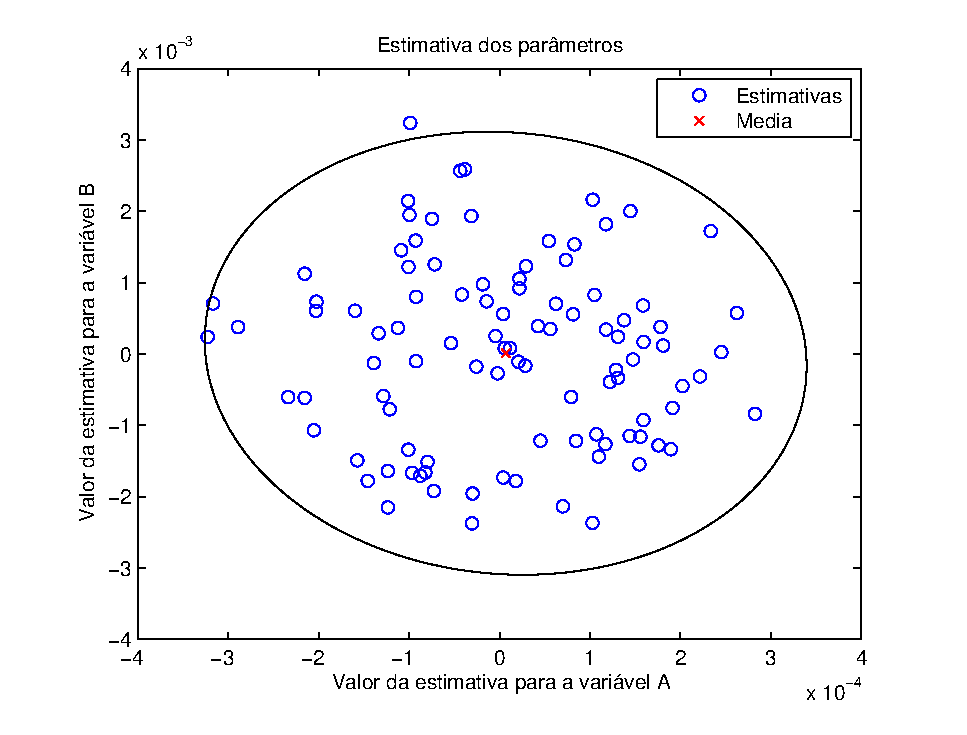
\includegraphics[width=0.8\columnwidth]{figures/si_covar_elipse.eps}
	\caption{Estimativas de um sistema e a regi�o de confian�a para $\chi$ de 95\%}
	\label{fig:si_covar_elipse}
\end{figure}


%===============================================================================
\section{Projeto de Experimento}
\label{sec:si_project_experiments}
%===============================================================================

Projeto de experimentos pode ser entendido como o procedimento para que se escolha o melhor 
sinal de entrada para a identifica��o dos par�metros desejados para o experimento. 
Desta forma muitas vari�veis podem ser levadas em considera��o, refletindo em propriedades que
podem ou n�o ser o foco do projeto de experimentos.

Uma forma de organizar o projeto de experimento � desenvolve-lo como um problema de otimiza��o 
convexa, onde entre muitas vantagens est� o fato de que � poss�vel a utiliza��o de m�todos matem�ticos
para o seu c�lculo e sua formula��o pode ser feita por LMI ({\it{Linear Matrix Inequality}}. Em \cite{jasson}
este t�pico � explorado em mais profundidade, sendo aqui apenas apresentado a sua ideia b�sica.

%===============================================================================
\subsection{Modelagem como um problema de otimiza��o}
\label{sec:si_project_optimization}
%===============================================================================

O problema de projeto de experimento pode ser considerado como uma forma geral apresentada em \eqref{eq:si_project_optimization}

\begin{equation}
\begin{matrix}
\underset{\Phi_{\chi_0}}{\text{minimize}} &  & \text{Objetivo}\\ 
\text{Sujeito a:} &  & \text{Requisitos de qualidade}\\ 
 &  & \text{Requisitos de sinais}
\end{matrix}
\label{eq:si_project_optimization}
\end{equation}

De forma geral os requisitos de qualidades s�o fun��es da covari�ncia de $P$. Por esta raz�o � natural usar
o espectro da entrada $\Phi_u$ e eventualmente o espectro cruzado $\Phi_{ue}$ como vari�veis do projeto.
A inclus�o de limita��es nos sinais e sua inclus�o como vari�veis de projeto s�o �teis para evitar que se chegue
em resultados onde a energia de entrada precise ser infinita para se obter os crit�rios desejados, ou largura
de banda que n�o s�o facilmente ating�veis em projetos reais. \cite{jasson}



%===============================================================================
\section{Considera��es Finais}
\label{sec:si_conclusions}
%===============================================================================

%===============================================================================



% ===============================================================================
\section{Virtual reference feedback tuning}
\label{sec:dbcd_vrft}
% ===============================================================================

% Em aplica��es pr�ticas, a descri��o matem�tica da planta n�o � dispon�vel e o sistema deve ser identificado
% baseado nas medidas obtidas deste sistema. Este assunto tem atra�do a aten��o de diversos engenheiros de
% controle desde 1940 com o pioneiro trabalho de Ziegler e Nichols (1942) com ajuste de controladores PID
% industriais. Depois do trabalho de Ziegler e Nichols diversos trabalhos surgiram, muitos em formas de
% aperfei�oamento e extens�es das t�cnicas j� apresentadas, e algumas com desenvolvimentos em novas dire��es
% (\cite{mcmillan1983tuning}, \cite{Haalman1965}). A caracter�stica principal destes m�todos � que eles podem
% ser facilmente utilizados: simples experimentos sobre a planta s�o executados e simples regras 
% s�o aplicadas sobre os dados obtidos. \cite{campi_leccini_savaresi2002}


VRFT do ingl�s {\it{Virtual reference feedback tuning}} � um m�todo direto para identifica��o de
controladores, ou seja, n�o � necess�rio o conhecimento ou identifica��o da planta para que este m�todo seja
utilizado. O m�todo se baseia na utiliza��o de apenas um conjunto de dados, n�o necessitando de experimentos
espec�ficos. O procedimento procura pelo ponto �timo do crit�rio escolhido para a identifica��o do controlador.
\cite{campi_savaresi2000}

Diferentemente de m�todos iterativos, o VRFT n�o recai sobre m�nimos locais, sempre procurando o m�nimo
global do crit�rio escolhido, sob condi��es ideais:

\begin{itemize}
  \item O sistema n�o � afetado por ru�do, ou seja, $\sigma_e^2(t)=0$.
  \item O controlador ideal $C_d(z) \in C(z, \theta)$.
  \item O controlador � parametrizado linearmente. 
\end{itemize}

O controlador a ser identificado pode ser parametrizado como abaixo:

\begin{equation}
C(z,\theta)=\beta^T(z)\theta
\label{eq:vrft_method_controller}
\end{equation}
onde $\beta(z) = \left [ \beta_1(z)\;\; \beta_2(z)\;\; \cdots \;\; \beta_n(z)\right ]^T$ � um vetor
linear de fun��es de transfer�ncias de tempo discreto e $\theta$ � o vetor de par�metros a ser estimado.

O problema de identifica��o do controlador consiste em encontrar um $\hat{\theta}$ que minimize o
crit�rio performance \eqref{eq:dbcd_def_track_error}, replicado abaixo:

\begin{equation}
J_y(\theta)\overset{\underset{\mathrm{\Delta}}{\,}}{=}  \bar{E} \left [ y(t)-y_d(t) \right ]^2 = \bar{E}\left [
(T(z,\theta)-T_d(z))r(t) \right ]^2
\nonumber
\end{equation}
que � dependente do modelo de refer�ncia escolhido. 

Apenas alguns m�todos genuinamente diretos s�o encontrados na literatura, dois destes s�o VRFT e IFT. Mesmo
estes dois m�todos pertencendo uma a mesma classe, algumas difer�n�as significativas existem e podem ser ressaltadas:
\cite{campi_savaresi2000}

\begin{itemize}
	\item {\it{IFT}} � baseado em um m�todos de gradiente decrescente e al�m disso � uma t�cnica
	iterativa. Usualmente este m�todo converge para o m�nimo local mais pr�ximo das condi��es iniciais.
	Ele requer experimentos espec�ficos sobre a planta, com entradas espec�ficas.
	\item {\it{VRFT}} � um procedimento n�o iterativo que procura pelo m�nimo global do crit�rio de
	performance \eqref{eq:dbcd_def_track_error}. Este m�todo n�o requer experimentos espec�ficos sobre
	a planta, podendo inclusive utilizar os dados do funcionamento normal do sistema.
\end{itemize}

%===============================================================================
\subsection{O m�todo}
\label{sec:dbcd_vrft_framework}
%===============================================================================

Nesta se��o ser� apresentado uma breve descri��o de como funciona o algoritmo para obten��o do controlador
utilizando o m�todo VRFT. Para maiores detalhes e discuss�es aprofundadas � indicada a leitura de
\cite{campi_savaresi2000, campi_leccini_savaresi2002, campestrini_nonminumum_phase, bazanella_datadriven}.

Suponha que o controlador $C(z, \theta)$ resulta um sistema em malha fechada cuja fun��o de
transfer�ncia � dada por $T_d(z)$. Desta forma, se $T_d(z)$ for excitado com qualquer sinal $r(t)$,
sua sa�da ser� $T_d(z)r(t)$. Uma premissa para que o sistema em malha fechada tenha a mesma
fun��o de transfer�ncia que o modelo de refer�ncia � que a sa�da dos dois sejaM a mesma para um dado
sinal $\bar{r}(t)$.

Baseado no sinal medido $y(t)$, considera-se um sinal $\bar{r}(t)$ tal que $T_d(z)\bar{r}(t)=y(t)$.
Esta refer�ncia � conhecida como {\it{virtual}} pois ela n�o existe e n�o foi utilizada para gerar o
sinal $y(t)$. A figura (\ref{fig:vrft_method_cl}) apresenta o sistema em malha fechada e os sinais
presentes.

\begin{figure}[htbp]
\center
%\scalebox{1} % Change this value to rescale the drawing.
%{
\begin{pspicture}(0,-1.4292188)(9.02,1.4692187)
\pscircle[linewidth=0.04,linestyle=dashed,dash=0.16cm 0.16cm,dimen=outer](1.4,0.97078127){0.2}
\psframe[linewidth=0.04,linestyle=dashed,dash=0.16cm 0.16cm,dimen=outer](4.8,1.3707813)(3.0,0.57078123)
\psframe[linewidth=0.04,dimen=outer](7.6,1.3707813)(6.0,0.57078123)
\psline[linewidth=0.04cm,arrowsize=0.05291667cm 2.0,arrowlength=1.4,arrowinset=0.4]{->}(0.0,0.97078127)(1.2,0.97078127)
\psline[linewidth=0.04cm,linestyle=dashed,dash=0.16cm 0.16cm,arrowsize=0.05291667cm 2.0,arrowlength=1.4,arrowinset=0.4]{->}(1.6,0.97078127)(3.0,0.97078127)
\psline[linewidth=0.04cm,arrowsize=0.05291667cm 2.0,arrowlength=1.4,arrowinset=0.4]{->}(4.8,0.97078127)(6.0,0.97078127)
\psline[linewidth=0.04cm](7.6,0.97078127)(9.0,0.97078127)
\psline[linewidth=0.04cm,linestyle=dashed,dash=0.16cm 0.16cm,arrowsize=0.05291667cm 2.0,arrowlength=1.4,arrowinset=0.4]{<-}(1.4,0.7707813)(1.4,-0.02921875)
\psline[linewidth=0.04cm,linestyle=dashed,dash=0.16cm 0.16cm](1.4,-0.02921875)(8.4,-0.02921875)
\psline[linewidth=0.04cm,linestyle=dashed,dash=0.16cm 0.16cm](8.4,-0.02921875)(8.4,0.97078127)
\usefont{T1}{ptm}{m}{n}
\rput(1.1126562,1.2807813){+}
\usefont{T1}{ptm}{m}{n}
\rput(1.6473438,0.68078125){-}
\usefont{T1}{ptm}{m}{n}
\rput(0.47,1.2707813){\small $\bar{r}(t)$}
\usefont{T1}{ptm}{m}{n}
\rput(3.99,0.97078127){\small $C(z, \theta)$}
\usefont{T1}{ptm}{m}{n}
\rput(6.76,0.9507812){\small $G_0(z)$}
\usefont{T1}{ptm}{m}{n}
\rput(5.51,1.2707813){\small $u(t)$}
\usefont{T1}{ptm}{m}{n}
\rput(2.25,1.2707813){\small $\varepsilon (t)$}
\usefont{T1}{ptm}{m}{n}
\rput(8.3,1.2707813){\small $y(t)$}
\psframe[linewidth=0.04,dimen=outer](6.0,-0.62921876)(3.8,-1.4292188)
\usefont{T1}{ptm}{m}{n}
\rput(4.91,-1.0492188){\small $T_d^{-1}(z)$}
\psline[linewidth=0.04cm](9.0,0.97078127)(9.0,-1.0292188)
\psline[linewidth=0.04cm](9.0,-1.0292188)(6.0,-1.0292188)
\psline[linewidth=0.04cm](3.8,-1.0292188)(0.0,-1.0292188)
\psline[linewidth=0.04cm](0.0,-1.0292188)(0.0,0.97078127)
\end{pspicture} 
%}
\caption{Diagrama de blocos para o m�todo VRFT. S�o destacados os sinais reais $u(t)$ e $y(t)$ al�m dos sinais virtuais
$\varepsilon (t)$ e $\bar{r}(t)$. Em pontilhado est� o controlador que quando aplicado sobre a malha, faz com que o
sistema se comporte como desejado: $T_d(z)$.}
\label{fig:vrft_method_cl}
\end{figure}

O sinal $\varepsilon(t)$ � o erro entre os sinais $y(t)$ e $\bar{r}(t)$. Sabe-se que quando a planta �
excitada com o sinal $u(t)$, o sinal $y(t)$ � obtido. Analogamente para um controlador, quando este �
excitado com o sinal $\varepsilon(t)$, o sinal $u(t)$ � obtido. A tarefa do m�todo VRFT � encontrar este
controlador, com os sinais $u(t)$ e $\varepsilon(t)$ que s�o conhecidos, a tarefa reduz-se a um problema de
identifica��o. Comumente, usa-se um pr�-filtro nos dados coletados. A ideia principal do uso deste
filtro ser� explicada posteriormente na se��o (\ref{sec:dbcd_vrft_framework_filter}). 

O algoritmo pode ser descrito pelos passos a seguir \cite{campi_savaresi2000}:

\begin{enumerate}
	\item Filtram-se os sinais de entrada e sa�da com algum filtro $L(z)$:

\begin{equation}
y_L (t)=L(z)y(t), \;\;\; u_L (t)=L(z)u(t) 
\label{eq:vrft_method_algorithm_filter_io}
\end{equation}

\begin{equation}
\varepsilon_L (t)=L(z)\varepsilon (t)=\bar{r}_L (t)-y_L (t) 
\nonumber
\end{equation}


\item Encontra-se um sinal de refer�ncia $\bar{r}_L (t)$ no qual a sa�da do modelo de refer�ncia
$T_d(z)$ seja exatamente $y_L (t)$ quando alimentado pelo sinal:

\begin{equation}
y_L (t)=T_d(z) \bar{r}_L (t)
\label{eq:vrft_method_algorithm_ref}
\end{equation}

\item Seleciona-se o vetor de par�metros do controlador $\hat{\theta}$ que minimize o crit�rio:

\begin{equation}
J_{VR}^N(\theta)=\frac{1}{N}\sum_{t=1}^{N}(u_L(t)-\varphi_L^T(t)\theta)^2
\label{eq:vrft_method_algorithm_criter}
\end{equation}

\begin{equation}
\varphi_L(t)=\beta(z)\varepsilon_L(t)
\nonumber
\end{equation}

Desde que \eqref{eq:vrft_method_algorithm_criter} seja quadr�tica em $\theta$ o vetor de par�metros
$\hat{\theta}$ que minimiza esta fun��o custo pode ser calculado por:

\begin{equation}
\hat{\theta}= \left [ \sum_{t=1}^{N}\varphi_L(t) \varphi_L(t)^T\right ]^{-1}
\sum_{t=1}^{N}\varphi_L(t) u_L(t)
\label{eq:vrft_method_algorithm_result}
\end{equation}

\end{enumerate}

Com o int�ito de exemplificar, na Figura (\ref{fig:vrft_cost_functions}) � apresentado uma curva da fun��o custo
$J_y(\theta)$ de um sistema hipot�tico, e a fun��o custo proposta pelo m�todo VRFT $J_{VR}(\theta)$, a qual � quadr�tica em $\theta$.
Ao tentar encontrar o ponto de m�nimo da curva $J_y(\theta)$ pode-se recair em algum m�nimo local, o que n�o acontece 
para a curva  $J_{VR}(\theta)$.

\begin{figure}[htbp]
\center
% Generated with LaTeXDraw 2.0.8
% Mon Jul 02 22:05:15 BRT 2012
% \usepackage[usenames,dvipsnames]{pstricks}
% \usepackage{epsfig}
% \usepackage{pst-grad} % For gradients
% \usepackage{pst-plot} % For axes
\scalebox{0.75} % Change this value to rescale the drawing.
{
\begin{pspicture}(0,-4.62)(11.799063,4.62)
\psbezier[linewidth=0.04](0.9,3.3)(2.1,3.2)(2.0225368,2.3742967)(2.1565964,1.5166456)(2.290656,0.6589943)(2.616248,-1.3127834)(3.008854,-0.5402044)(3.4014597,0.23237456)(3.6584003,0.8693678)(3.811938,0.20167358)(3.9654756,-0.4660206)(4.5199084,-3.4794219)(5.1017394,-3.533306)(5.68357,-3.5871902)(8.0,1.8)(9.5,3.2)
\psbezier[linewidth=0.04,linestyle=dashed,dash=0.16cm 0.16cm](0.4,2.2)(2.2,-2.6)(3.960841,-3.4989967)(5.12,-3.54)(6.279159,-3.5810034)(9.3,-1.9)(10.6,1.9)
\psline[linewidth=0.04cm,arrowsize=0.05291667cm 4.0,arrowlength=1.4,arrowinset=0.4]{<-}(1.1,4.6)(1.2,-4.6)
\psline[linewidth=0.04cm,arrowsize=0.05291667cm 4.0,arrowlength=1.4,arrowinset=0.4]{->}(0.0,-3.9)(11.3,-3.9)
\psline[linewidth=0.04cm,linestyle=dotted,dotsep=0.16cm](5.1,-4.0)(5.0,3.1)
\usefont{T1}{ppl}{m}{n}
\rput(5.114531,-4.19){$\theta^*$}
\usefont{T1}{ppl}{m}{n}
\rput(11.014531,-4.19){$\theta$}
\usefont{T1}{ppl}{m}{n}
\rput(0.5545313,4.01){$J(\theta)$}
\usefont{T1}{ppl}{m}{n}
\rput(2.5545313,2.71){$J_y$}
\usefont{T1}{ppl}{m}{n}
\rput(3.2145312,-1.79){$J_{VR}$}
\end{pspicture} 
}
\caption{Gr�fico da fun��o custo de algum sistema hipot�tico e a respectiva fun��o custo proposta plo m�todo VRFT que �
mais simples de encontrar o ponto de m�nimo pois � quadr�tica em $\theta$, n�o recaindo em m�nimos locais. O valor
$\theta^*$ � o ponto de m�nimo de ambas as fun��es custo, logo, minimizando a fun��o custo $J_{VR}(\theta)$ � o
equivalente a minimizar $J_y(\theta)$ sob condi��es ideais.}
\label{fig:vrft_cost_functions}
\end{figure}

%===============================================================================
\subsection{Utiliza��o do Filtro $L(z)$}
\label{sec:dbcd_vrft_framework_filter}
%===============================================================================

Considerando a fun��o custo $J_{y}(\theta)$ apresentada em \eqref{eq:dbcd_def_track_error} e o
crit�rio do m�todo de refer�ncia virtual $J_{VR}(\theta)$ apresentado em \eqref{eq:vrft_method_algorithm_criter} serem
diferentes fora de situa��es ideais. A escolha correta do filtro $L(z)$ propicia que estas duas equa��es tenham m�nimos
muito pr�ximos \cite{campi_leccini_savaresi2002}.

A utiliza��o do filtro � de grande import�ncia em situa��es onde a escolha do modelo $C(z,\theta)$ n�o consegue
representar a totalidade do controlador �timo ($C_d(z)$) que quando aplicado em conjunto com a planta proporciona a
exata resposta desejada pela escolha de $T_d(z)$, ou seja:

\begin{equation}
C_d(z) \notin C(z, \theta)
\nonumber
\end{equation}

Aplicando o teorema de Perseval  para a fun��o custo de seguimento de refer�ncia:

\begin{equation}
J_y(\theta)=\bar{E}\left [ (T(z,\theta)-T_d(z))r(t) \right ]^2
\nonumber
\end{equation}
e usando as rela��es de malha fechada:

\begin{equation}
T_d(z)=\frac{C_d(z)G_0(z)}{1+C_d(z)G_0(z)}\;\;\;\; T(z, \theta)=\frac{C(z, \theta)G_0(z)}{1+C(z, \theta)G_0(z)}
\nonumber
\end{equation}

Resultam na seguinte express�o no dominio da frequ�ncia para a fun��o custo:

\begin{equation}
J_y(\theta)=\frac{1}{2\pi}\int_{-\pi}^{\pi}\left | \frac{G_0(e^{j\omega})C(e^{j\omega},
\theta)}{1+G_0(e^{j\omega})C(e^{j\omega},\theta)}-\frac{G_0(e^{j\omega})C_d(e^{j\omega})}{1+G_0(e^{j\omega})C_d(e^{j\omega})} \right |^2 \Phi_r(e^{j\omega})d\omega
\nonumber
\end{equation}

Desenvolvendo esta express�o, pode-se descreve-la mais compactamente como:

\begin{eqnarray}\nonumber
J_y(\theta)&=&\frac{1}{2\pi}\int_{-\pi}^{\pi}\left | G_0(e^{j\omega}) \right |^2 \left | S(e^{j\omega},\theta) \right |^2\left | S_d(e^{j\omega}) \right |^2 \\
&&  \times \left | C(e^{j\omega},\theta)-C_d(e^{j\omega}) \right |^2 \Phi_r(e^{j\omega})d\omega
\label{eq:dbcd_vrft_jy_cost}
\end{eqnarray}

Adiciona-se o filtro $L(z)$ � fun��o custo do VRFT, $J_{VR}(\theta)$:

\begin{equation}
J_{VR}(\theta)=\bar{E}\left [ L(z)(u(t)-C(z,\theta)\bar{\varepsilon}(t)) \right ]^2
\nonumber
\end{equation}
e usando as rela��es:

\begin{equation}
1-T_d(e^{j\omega})=S_d(e^{j\omega})
\nonumber
\end{equation}
e

\begin{equation}
\frac{T_d(e^{j\omega})}{G_0(e^{j\omega})}=C_d(e^{j\omega})S_d(e^{j\omega})
\nonumber
\end{equation}
pode-se ent�o reescrever a fun��o custo do VRFT como :


\begin{eqnarray}\nonumber
J_{VR}(\theta)&=&\frac{1}{2\pi}\int_{-\pi}^{\pi}\left | L(e^{j\omega}) \right |^2 \frac{\left | G_0(e^{j\omega}) \right
|^2 \left | S_d(e^{j\omega}) \right |^2}{\left | T_d(e^{j\omega}) \right |^2}\\ 
 && \times \left | C_d(e^{j\omega})- C(e^{j\omega},\theta) \right |^2 \Phi_u(e^{j\omega})d\omega  
\label{eq:dbcd_vrft_jvr_cost}
\end{eqnarray}

Comparando agora \eqref{eq:dbcd_vrft_jy_cost} e \eqref{eq:dbcd_vrft_jvr_cost}, observa-se que quando $C_d(z) \in
C(z,\theta)$ as duas fun��es custo s�o iguais, possuindo tamb�m o mesmo m�nimo. Quando $C_d(z) \notin C(z,\theta)$
nenhum dos crit�rios desaparece e o ponto de m�nimo depende de v�rios fatores dentro da integral. Se os fatores dentro dos dois
integrandos s�o diferentes, n�o existe motivos para esperar que os dois custos dejam o mesmo.
\cite{bazanella_datadriven}

Existe entretanto o parametro livre que foi incluido � fun��o custo do VRFT que pode ser escolhido a fim de aproximar
estes dois integrandos: o filtro $L(z)$. Para fazer com que $J_{VR}(\theta)=J_y(\theta)$, � suficiente escolher
$L(e^{j\omega})$ como:

\begin{equation}
\left | L(e^{j\omega}) \right |^2=\left | T_d(e^{j\omega}) \right |^2\left | S(e^{j\omega},\theta) \right
|^2\frac{\Phi_r(e^{j\omega})}{\Phi_u(e^{j\omega})}, \;\;\;\; \forall\omega \in \left [ -\pi; \pi \right ]
\label{eq:dbcd_vrft_filter_l}
\end{equation}
onde $\Phi_r(e^{j\omega})$ representa o espectro do sinal real da refer�ncia $r(t)$ e $\Phi_u(e^{j\omega})$ representa o
espectro do sinal aplicado sobre o sistema, medido durante o experimento do VRFT.

O c�lculo do filtro apresentado em \eqref{eq:dbcd_vrft_filter_l} requer do conhecimento da fun��o $S(z,\theta)$, que
algumas vezes pode n�o ser conhecida. Ent�o a implementa��o deste filtro ir� recair em alguma aproxima��o desta fun��o
de transfer�ncia. Quanto melhor for a aproxima��o, mais pr�ximos ser�o os m�nimos das fun��es custo $J_y(\theta)$ e
$J_{VR}(\theta)$. \cite{bazanella_datadriven}

Entretanto esta n�o � a �nica escolha sens�vel para a aproxima��o de $S(z,\theta)$, VRFT usa invariavelmente o seguinte:

\begin{equation}
\left | S(e^{j\omega},\theta) \right |^2\approx \left | S_d(e^{j\omega}) \right |^2=\left | 1-T_d(e^{j\omega}) \right
|^2
\label{eq:dbcd_vrft_sensible_s}
\end{equation}
o que aparenta ser uma aproxima��o razoavel, uma vez que � esperado que as duas fun��es sensibilidades em
\eqref{eq:dbcd_vrft_sensible_s} sejam pr�ximas ao redor do ponto de m�nimo. Usando esta aproxima��o, a fun��o de
transfer�ncia do filtro pode ser obtida por:

\begin{equation}
\left | L(e^{j\omega}) \right |^2=\left | T_d(e^{j\omega}) \right |^2\left | 1-T_d(e^{j\omega},\theta) \right
|^2\frac{\Phi_r(e^{j\omega})}{\Phi_u(e^{j\omega})}, \;\;\;\; \forall\omega \in \left [ -\pi; \pi \right ]
\label{eq:dbcd_vrft_filter_l_vrft}
\end{equation}

Para o caso onde $C_d \in C(z, \theta)$ a escolha de $L(z)$ n�o afeta o resultado, usualmente
escolhe-se ent�o $L(z)=1$.\cite{campi_leccini_savaresi2002}

Com o fltro $L(z)$ calculado como em \eqref{eq:dbcd_vrft_filter_l_vrft}, o valor assint�tico de $\theta$ pode ser
escrito como:

\begin{equation}
\theta_*=\bar{E}\left [ \varphi_L(t)\varphi_L(t)^T  \right ]^{-1}\bar{E}\left [ \varphi_L(t)u_L(t)  \right ]
\label{eq:dbcd_vrft_filter_estim}
\end{equation}
onde $\varphi_L(t)=L(z)\varphi(t)$ e $u_L(t)=L(z)u(t)$. O c�lculo real para obter os par�metros da estimativa � dado
por:

\begin{equation}
\theta=\left [ \sum_{t=1}^{N}\varphi_L(t)\varphi_L^T(t) \right ]^{-1} \sum_{t=1}^{N}\varphi_L(t)u_L(t)
\label{eq:dbcd_vrft_filter_estim_N}
\end{equation}
e na aus�ncia de ru�do, $\theta$ � igual ao valor de $\theta_*$ apresentado em \eqref{eq:dbcd_vrft_filter_estim}.

Na figura \ref{fig:vrft_cost_functions_L} um exemplo hipot�tico, onde o valor de $\theta$ que minimiza $J_{VR}(\theta)$ se
aproxima do valor de m�nimo de $J_y(\theta)$ com a utiliza��o do filtro $L(z)$. Tamb�m observa-se que a curva de
$J_{VR}(\theta)$ quando o filtro � aplicado apresenta uma redu��o na sua concavidade, fazendo com que o valor de m�nimo
na curva encontrado pelo algoritmo seja menos preciso, aumentando o a vari�ncia das estimativas, enquanto reduz o erro
de polariza��o.

\begin{figure}[htbp]
\center
% Generated with LaTeXDraw 2.0.8
% Tue Jul 03 00:08:46 BRT 2012
% \usepackage[usenames,dvipsnames]{pstricks}
% \usepackage{epsfig}
% \usepackage{pst-grad} % For gradients
% \usepackage{pst-plot} % For axes
\scalebox{0.75} % Change this value to rescale the drawing.
{
\begin{pspicture}(0,-3.97)(11.489062,3.97)
\psbezier[linewidth=0.04,linestyle=dashed,dash=0.16cm 0.16cm](0.59,-0.85)(1.39,-1.95)(3.950841,-2.6489966)(5.11,-2.69)(6.269159,-2.7310033)(8.69,-2.05)(9.69,-0.95)
\psline[linewidth=0.04cm,arrowsize=0.05291667cm 4.0,arrowlength=1.4,arrowinset=0.4]{<-}(1.39,3.95)(1.39,-3.95)
\psline[linewidth=0.04cm,arrowsize=0.05291667cm 4.0,arrowlength=1.4,arrowinset=0.4]{->}(0.59,-3.25)(11.09,-3.25)
\usefont{T1}{ppl}{m}{n}
\rput(10.704532,-3.54){$\theta$}
\usefont{T1}{ppl}{m}{n}
\rput(0.88453126,3.36){$J(\theta)$}
\usefont{T1}{ppl}{m}{n}
\rput(1.9445312,-0.04){$J_y$}
\usefont{T1}{ppl}{m}{n}
\rput(4.804531,1.16){$J_{VR}$}
\psbezier[linewidth=0.04](0.79,1.15)(0.79,0.35)(2.8950949,-2.049184)(3.89,-2.15)(4.884905,-2.2508159)(4.788093,-1.547449)(5.59,-0.95)(6.3919067,-0.35255104)(6.676079,-1.3078374)(7.19,-0.45)(7.7039213,0.40783736)(7.61,0.85)(8.01,1.71)(8.41,2.57)(9.09,2.89)(9.59,3.05)
\psbezier[linewidth=0.04,linestyle=dotted,dotsep=0.16cm](3.69,1.55)(4.49,0.45)(5.950841,-1.8489966)(7.11,-1.89)(8.269159,-1.9310033)(10.09,0.75)(10.99,1.85)
\usefont{T1}{ppl}{m}{n}
\rput(7.8545313,-2.54){$J_{VR}^L$}
\psdots[dotsize=0.24,dotstyle=asterisk](5.29,-2.71)
\psdots[dotsize=0.24,dotstyle=asterisk](7.15,-1.91)
\psdots[dotsize=0.24,dotstyle=asterisk](4.05,-2.17)
\end{pspicture} 
}
\caption{Exemplo hipot�tico de fun��es custo na sitau��o onde o controlador ideal n�o consegue ser representado pelo
modelo. Situa��o esta que o uso do filtro $L(z)$ agrega valor reduzindo o erro de polariza��o da estimativa -
Observa-se a aproxima��o do valor de m�nimo das fun��es custo pelo uso do filtro ($J(\theta)_{VR}^L$).}
\label{fig:vrft_cost_functions_L}
\end{figure}


%===============================================================================
\subsection{Dados corrompidos por ru�do}
\label{sec:dbcd_vrft_framework_noise}
%===============================================================================

Nesta se��o ser� apresentado brevemente o comportamento do m�todo quando o sinal $y(t)$ �
corrompido por um ru�do aditivo como:

\begin{equation}
\tilde{y}(t)=G_0(z)u(t) + \nu(t)
\label{eq:vrft_framework_noise_y}
\end{equation}

Assume-se que o sinal $u(t)$ e $\nu(t)$ sejam descorrelacionados e tamb�m que os dados s�o coletados
com a planta trabalhando em la�o aberto \cite{campi_leccini_savaresi2002}. A ideia estendida
de dados coletados com a planta em la�o fechado, podem ser encontradados em \cite{lecchini}.

Ao aplicar o algoritmo descrito na se��o (\ref{sec:dbcd_vrft_framework}) com dados sujeitos a ru�dos, o
resultado obtido possui erro de polariza��o. Isso pode ser compreendido analisando a express�o do crit�rio
$J_{VR}(\theta)$ quando utiliza-se o sinal $\tilde{y}(t)$:

\begin{eqnarray}\nonumber
J_{VR}(\theta)&=&\frac{1}{2\pi} \int_{-\pi}^{\pi} \left | G_0(e^{j\omega}) \right |^2 \left |
 C(e^{j\omega},\theta)-C_d(e^{j\omega}) \right |^2 \left | 1-T_d(e^{j\omega}) \right |^2 \frac{\left | L(e^{j\omega})
 \right |^2}{\left | T_d(e^{j\omega}) \right |^2}  \Phi_u(e^{j\omega}) \\
 && + \frac{\left | C(e^{j\omega},\theta) \right  |^2}{\left | G_0(e^{j\omega}) \right |^2 \left | C_d(e^{j\omega})
 \right |^2}\left | L(e^{j\omega}) \right |^2\Phi _d \; d\omega
\label{eq:vrft_framework_noise_vr}
\end{eqnarray}
onde $\Phi_d$ � a densidade do espectro do ru�do.

Para que haja rejei��o a este rudo no m�todo, em \cite{campi_leccini_savaresi2002} foi sugerido a
adi��o da vari�vel instrumental $\zeta(t)$. Em \eqref{eq:vrft_framework_noise_iv} apresenta-se o
regressor deste instrumento:

\begin{equation}
\tilde{\varphi }_L(t)=\beta(z)L(z)\left ( T_d(z)^{-1}-1 \right )\tilde{y}(t)
\label{eq:vrft_framework_noise_iv}
\end{equation}

Os par�metros do controlador podem ent�o ser calculados como em:

\begin{equation}
\theta_{N}^{IV}=\left [ \sum_{t=1}^{N}\zeta(t) \tilde{\varphi}_L(t)^T \right ]^{-1}\left [ 
\sum_{t=1}^{N}\zeta(t)u_L(t) \right ]
\label{eq:vrft_framework_noise_theta_iv}
\end{equation}

S�o propostas duas alternativas para a escolha da vari�vel instrumental. A primeira garante
assintoticamente que $\theta_N^{IV}= \theta_0$, entretanto um experimento adicional �
requisitado. O segundo n�o garante, rigorosamente, $\theta_N^{IV}= \theta_0$ mas o erro
esperado � pequeno, al�m disso um segundo experimento n�o � necess�rio. \cite{campi_leccini_savaresi2002}

\begin{itemize}
	\item {\it{Experimento Repetido:}} Executa-se um segundo experimento com a mesma entrada $u(t)$,
	adquirindo-se a sa�da $\tilde{y}(t)'$. Como o ru�do entre um experimento e outro � independente,
	$\tilde{y}(t)$ e $\tilde{y}(t)'$ ser�o diferentes. Obt�m-se ent�o a vari�vel instrumental:
	
	\begin{equation}
	\zeta(y)=\beta(z)L(z)\left ( T_d(z)^{-1}-1 \right )\tilde{y}(t)'
	\nonumber
	\end{equation}
	
	\item {\it{Identifica��o da planta:}} Identifica-se a planta $G_0(z)$ com uma famil�a de modelos como $G(z,\theta_G)$ a
	partir do conjunto de dados $\left \{ u(t), \; \tilde{y}(t) \right \}_{t=1,..., N}$ e ent�o gera-se o sinal simulado
	$\hat{y}=G(z,\theta_G)u(t)$, obtendo a vari�vel instrumental como:

	\begin{equation}
	\zeta(y)=\beta(z)L(z)\left ( T_d(z)^{-1}-1 \right )\hat{y}(t)
	\nonumber
	\end{equation}
	
	Devido as incertezas na estimativa de $G(z,\theta_G)$, este segundo m�todo n�o garante que a
	estimativa tenda assintoticamente a $\theta_0$.
\end{itemize}

%===============================================================================
\subsection{Exemplos ilustrativos}
\label{sec:dbcd_vrft_examples}
%===============================================================================

Nesta se��o ser�o apresentados alguns exemplos ilustrativos da utiliza��o do m�todo do VFRT. Ser�o utilizados sistemas
lineares modelados pelas classes de modelos ARX e BJ quando o controlador $C(z, \theta)$ faz parte da classe de
controladores que representa completamente o controlador ideal e tamb�m um caso onde o controlador ideal $C_d(z)$ n�o
consegue ser presentado pela classe de controlador escolhida.

Nas identifica��es apresentadas a seguir ser� sempre utilizado um sinal PRBS de ordem 7.

%===============================================================================
\subsubsection{Controlador PI - sistema Box-Jenkins}
\label{sec:dbcd_vrft_examples_pi_bj}
%===============================================================================

Considere o sistema real definido como:

\begin{equation}
G_{ 0 }(z)=\frac { 0.5 }{ z-0.85 } ,\quad \quad \quad H_{ 0 }(z)=\frac { z }{
z-0.4 } 
\nonumber
\end{equation}

Este sistema pode ser compreendido como um sistema {\it{Box-Jenkins}} (BJ)
(Tabela (\ref{table:si_modeling_models})). Deseja-se que o sistema em malha
fechada comporte-se o mais pr�ximo poss�vel de:

\begin{equation}
T_d(z)=\frac { 0.4 }{ z-0.6 }
\label{eq:vrft_methos_ex_bj_M}
\end{equation}

Tem-se assim que o controlador ideal pode ser definido por:

\begin{equation}
C_d(z)=\frac{T_d(z)}{G_0(z)(1-T_d(z))} = \frac { 0.8(z - 0.85) }{ z-1 }
\label{eq:vrft_methos_ex_bj_cd}
\end{equation}

Observa-se que este controlador pode ser representado como um controlador {\it{PI}} como em: 

\begin{equation}
C(z, \theta)=\frac { \theta_1 z +\theta_2}{ z-1 }
\label{eq:vrft_methos_ex_bj_c}
\end{equation}

Escolheu-se \eqref{eq:vrft_methos_ex_bj_c} como sendo a classe de modelos a ser utilizada para a identifica��o do
controlador.

Utilizando o m�todo do VRFT para identifica��o do controlador quando este est� submetido a um ru�do $\sigma_e^2=0.005$
obt�m-se a estimativas dos par�metro s $\theta_1$ e $\theta_2$ apresentados na Figura (\ref{fig:vrft_bj_M10_var005})
com um resultado de 100 simula��es com $N=2540$ cada.

\begin{figure}[htbp]
	\center
	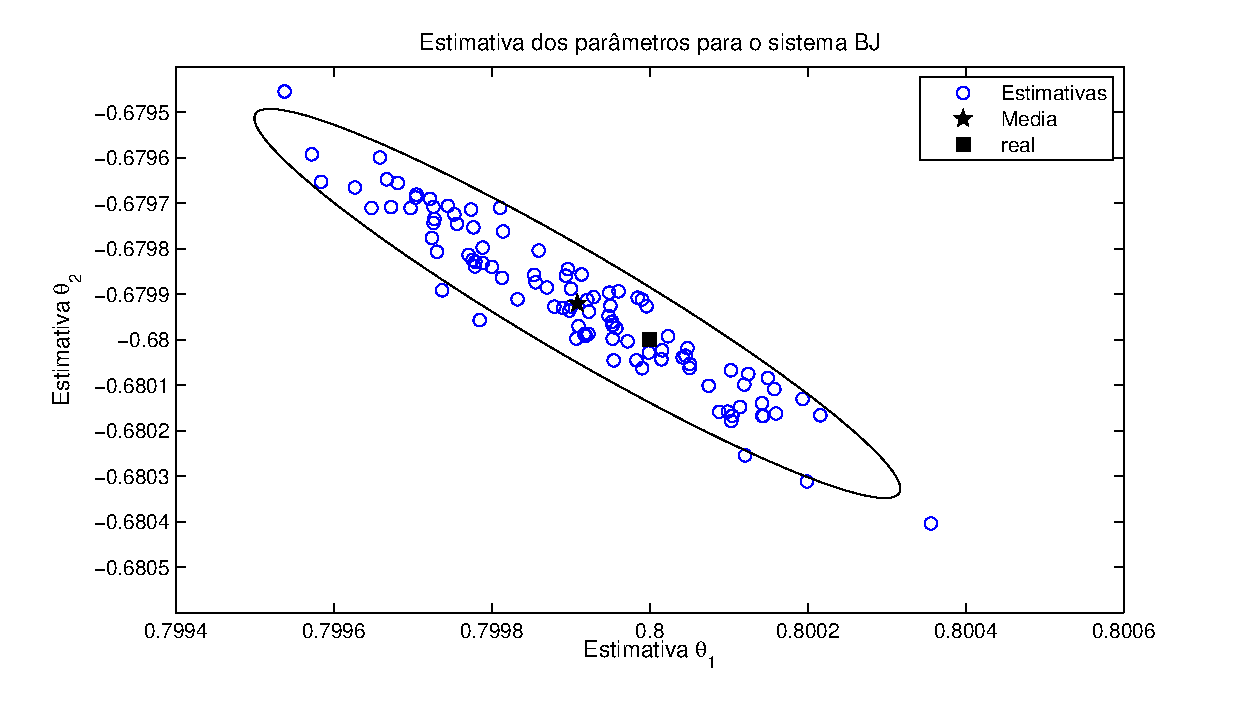
\includegraphics[width=0.95\columnwidth]{figures/vrft_bj_M10_var005.eps}
	\caption{Resultado das 100 estimativas de Monte Carlo dos par�metros $\theta_1$ e $\theta_2$ para o controlador
	apresentado em \eqref{eq:vrft_methos_ex_bj_c}. Adicionado a simula��o um ru�do aditivo de vari�ncia $\sigma_e^2=0.005$}
	\label{fig:vrft_bj_M10_var005}
\end{figure}

Os par�metros reais esperados para o controlador (equa��o \eqref{eq:vrft_methos_ex_bj_cd}) e a m�dia de todas
as estimativas $\hat{\theta}_N$ (valor representado por uma estrela na Figura (\ref{fig:vrft_bj_M10_var005})) n�o s�o os
mesmos. Em uma situa��o onde o erro de polariza��o das estimativas n�o existe, o aumento de N (n�mero de
amostras) implica que esta diferen�a diminui, tendendo a zero. Em um cen�rio onde h� erro de polariza��o, se 
aumentarmos a vari�ncia do ru�do do sistema, ser� observado um aumento desta diferen�a.

\begin{equation}
\lim_{N \rightarrow \infty }\hat{\theta}_N = \theta_0
\nonumber
\end{equation}

Na figura (\ref{fig:vrft_bj_M10_var02})  � apresentado o resultado para a estimativa de $\theta$ quando a vari�ncia do 
ru�do � quadruplicada ($\sigma_e^2=0.02$). Observa-se ent�o que o erro de polariza��o existe na estimativa. Como
descrito em \cite{campi_leccini_savaresi2002} quando o m�todo do VRFT � utilizado com ru�do nas amostras, a estimativa
� inevitavelmente polarizada. Na se��o (\ref{sec:dbcd_vrft_framework_noise}) foi sugerido o uso de vari�veis
instrumentais par para que este erro de polariza��o seja minimizado. Utilizou-se ent�o este m�todo e para um ru�do com
a mesma vari�ncia ($\sigma_e ^2=0.02$), o resultado �btido � o apresentado na Figura (\ref{fig:vrft_bj_M10_var02_iv}).

\begin{figure}[htbp] 
	\center 
	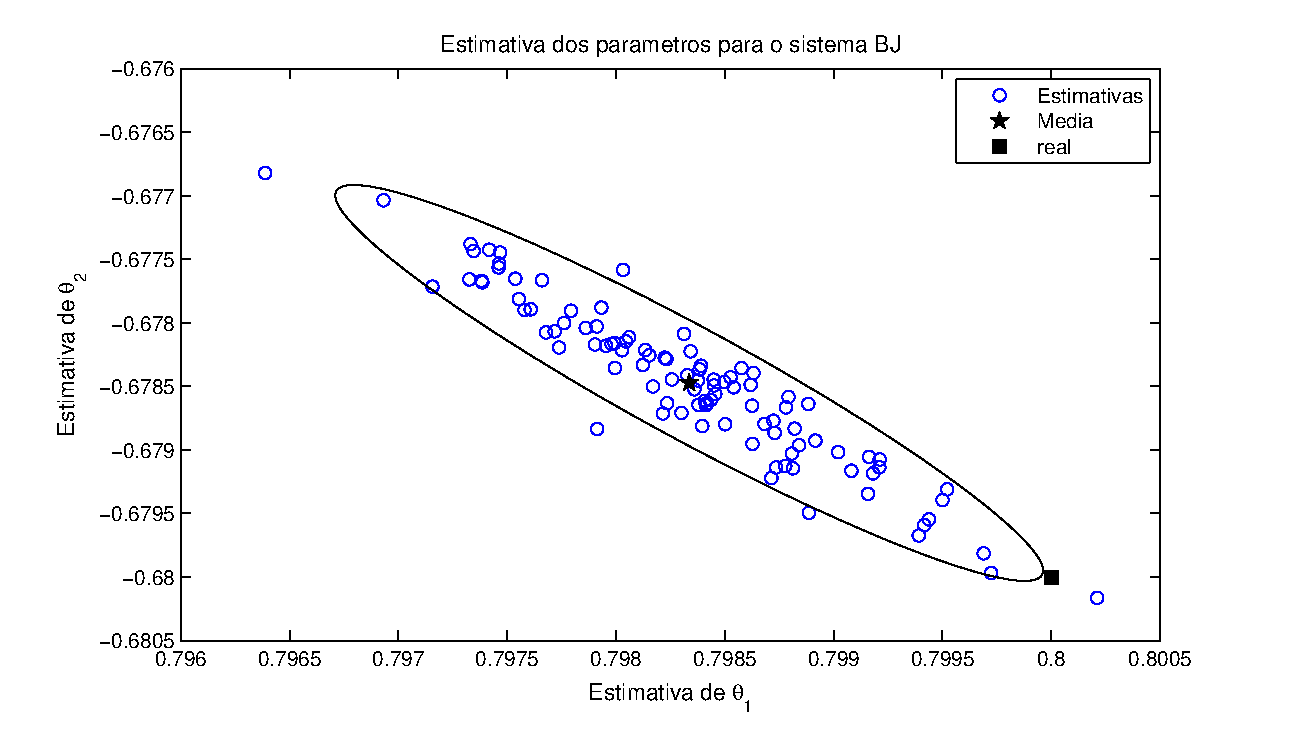
\includegraphics[width=0.95\columnwidth]{figures/vrft_bj_M10_var02.eps}
	\caption{100 estimativas Monte Carlo dos par�metros $\theta_1$ e $\theta_2$ para o controlador apresentado em
	\eqref{eq:vrft_methos_ex_bj_c} com um ru�do de vari�ncia de $\sigma_e^2=0.02$.}
	\label{fig:vrft_bj_M10_var02}
\end{figure}

\begin{figure}[htbp]
	\center
	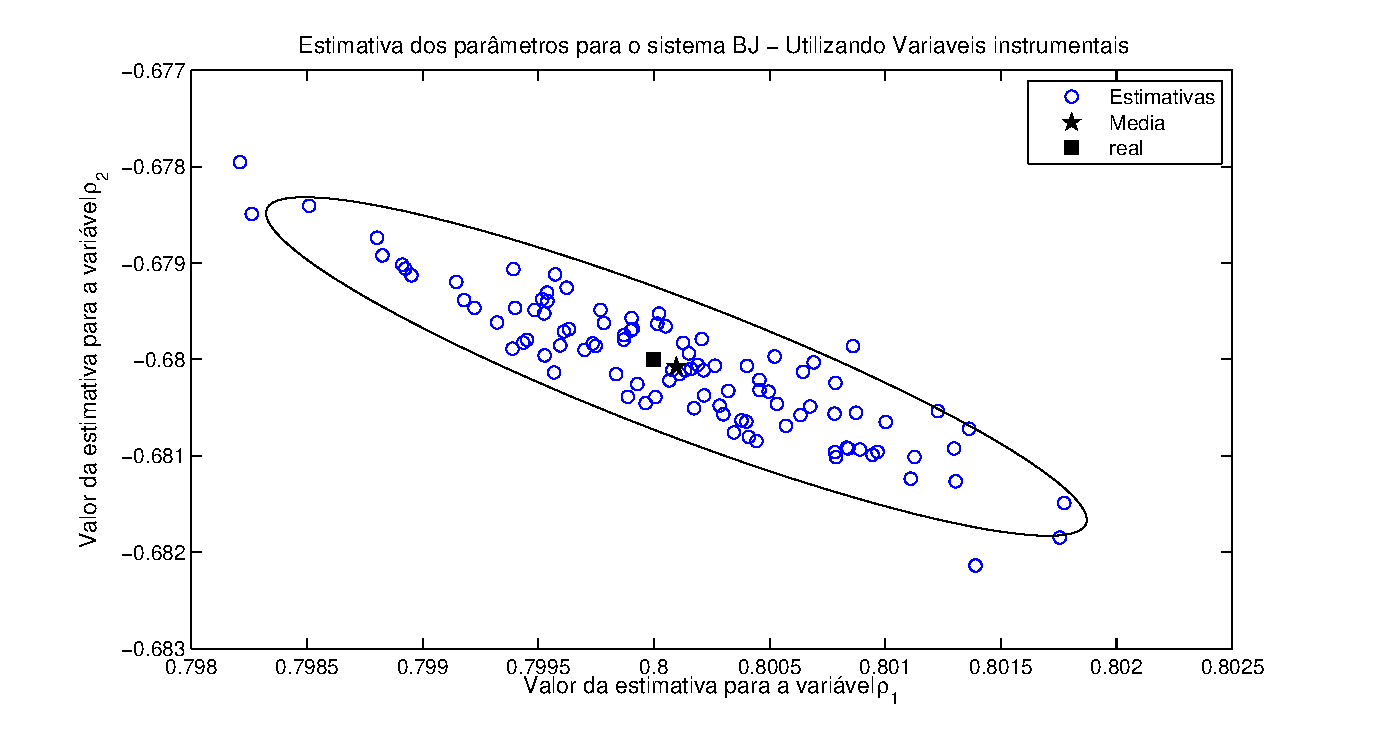
\includegraphics[width=0.95\columnwidth]{figures/vrft_bj_M10_var02_iv.eps}
	\caption{Resultado das 100 estimativas de Monte Carlo dos par�metros $\theta_1$ e $\theta_2$ para o
	controlador apresentado em \eqref{eq:vrft_methos_ex_bj_c} com vari�ncia do
	ru�do de 0.02. Utilizando vari�veis instrumentais para estimar os par�metros.}
	\label{fig:vrft_bj_M10_var02_iv}
\end{figure}

Observa-se que o erro de polariza��o foi minimizado e que o resultado obtido possui um custo $J_{VR}^N(\theta)
= 5.1242$ e a vari�ncia dos par�metros estimados foi de $0.5064\times10^{-6}$ para $\theta_1$ e de
$0.5495\times10^{-6}$ para $\theta_2$.

A fim de comparar o m�todo VRFT utilizando e n�o utilizando vari�veis instrumentais s�o apresentados abaixo as
Tabelas (\ref{table:vrft_method_bj}) e (\ref{table:vrft_method_bj_iv}) onde os custo $J_{y}$ e $J_{VR}^N$ s�o
apresentados para diferentes valores de vari�ncia do ru�do para o mesmo sistema BJ.

\begin{table*}[htbp]
\begin{center}
\caption{Valor dos custos $J_{VR}^N$ e $J_{y}$ al�m da vari�ncia das estimativas para diferentes valores de $\sigma_e^2$
quando o m�todo VRFT n�o utiliza vari�veis instrumentais para a estimativa dos par�metros $\theta$}
\label{table:vrft_method_bj}
\begin{tabular}{ccccc}
\hline
        Vari�ncia $\sigma_e^2$ & $J_{VR}^N(\theta)$ & $J_y(\theta)$ & M�dia $\theta_1$ & M�dia $\theta_2$  \\
\hline
	 0.1 	 & 	 4.87826e-02 	 & 	 2.15324e-02 	 & 	 0.76178 	 & 	 0.64466 \\ 
	 0.08 	 & 	 3.26789e-02 	 & 	 1.35688e-02 	 & 	 0.7759 	 & 	 0.65765 \\ 
	 0.06 	 & 	 1.80426e-02 	 & 	 7.86422e-03 	 & 	 0.78597 	 & 	 0.66715 \\ 
	 0.05 	 & 	 1.19341e-02 	 & 	 5.52796e-03 	 & 	 0.79017 	 & 	 0.67088 \\ 
	 0.04 	 & 	 7.54289e-03 	 & 	 3.65088e-03 	 & 	 0.79351 	 & 	 0.67396 \\ 
	 0.01 	 & 	 4.89481e-04 	 & 	 2.11052e-04 	 & 	 0.79962 	 & 	 0.67965 \\ 
	 0.008 	 & 	 3.25810e-04 	 & 	 1.83444e-04 	 & 	 0.79968 	 & 	 0.67969 \\ 
	 0.005 	 & 	 1.20816e-04 	 & 	 5.42193e-05 	 & 	 0.7999 	 & 	 0.67991 \\ 
	 0.003 	 & 	 4.73517e-05 	 & 	 2.28052e-05 	 & 	 0.79996 	 & 	 0.67996 \\ 
	 0.001 	 & 	 5.02347e-06 	 & 	 2.77267e-06 	 & 	 0.8 	     & 	 0.68 \\ 
\hline
\end{tabular}
\end{center}
\end{table*} 
   

\begin{table*}[htbp]
\begin{center}
\caption{Valor dos custos $J_{VR}^N$ e $J_{y}$ al�m da  vari�ncia das estimativas para diferentes valores de
$\sigma_e^2$ quando o m�todo VRFT utiliza vari�veis instrumentais para a estimativa dos par�metros $\theta$}
\label{table:vrft_method_bj_iv}
\begin{tabular}{ccccc}
\hline
        Vari�ncia $\sigma_e^2$ & $J_{VR}^N(\theta)$ & $J_{y}(\theta)$  & M�dia $\theta_1$ & M�dia $\theta_2$  \\
\hline
	 0.1 	 & 	 5.19132e-02 	 & 	 4.14964e-04 	 & 	 0.79936 	 & 	 0.67971 \\ 
	 0.08 	 & 	 3.31577e-02 	 & 	 2.96000e-04 	 & 	 0.80037 	 & 	 0.68007 \\ 
	 0.06 	 & 	 1.70932e-02 	 & 	 2.17256e-04 	 & 	 0.79989 	 & 	 0.67969 \\ 
	 0.05 	 & 	 1.27803e-02 	 & 	 3.14017e-05 	 & 	 0.80006 	 & 	 0.68005 \\ 
	 0.04 	 & 	 7.72145e-03 	 & 	 9.43578e-05 	 & 	 0.79996 	 & 	 0.68006 \\ 
	 0.01 	 & 	 5.00316e-04 	 & 	 3.20694e-05 	 & 	 0.80005 	 & 	 0.68003 \\ 
	 0.008 	 & 	 3.44326e-04 	 & 	 2.93508e-05 	 & 	 0.80001 	 & 	 0.68004 \\ 
	 0.005 	 & 	 1.19855e-04 	 & 	 6.96916e-06 	 & 	 0.79999 	 & 	 0.68 \\ 
	 0.003 	 & 	 4.22380e-05 	 & 	 6.33696e-06 	 & 	 0.80001 	 & 	 0.68001 \\ 
	 0.001 	 & 	 5.08709e-06 	 & 	 1.18016e-06 	 & 	 0.8 	 	 & 	 0.68 \\ 
\hline
\end{tabular}
\end{center}
\end{table*}

Utilizando vari�veis instrumentais observa-se que o custo $J_{y}(\theta)$ � significativamente mais baixo
quando comparado com o m�todo onde n�o s�o utilizadas vari�veis instrumentais, corroborando com o que foi apresentado na
se��o (\ref{sec:dbcd_vrft_framework_noise}).

%===============================================================================
\subsubsection{Controlador PID - sistema ARX}
\label{sec:dbcd_vrft_examples_pid_arx}
%===============================================================================

Considere o sistema real definido pefinido pelo modelo ARX:

\begin{equation}
G_{ 0 }(z)=\frac { z }{ (z-0.9)(z-0.8) } ,\quad \quad \quad H_{ 0 }(z)=\frac { z^2 }{ (z-0.9)(z-0.8) } 
\nonumber
\end{equation}

Deseja-se que o sistema em malha fechada comporte-se como:

\begin{equation}
T_d(z)=\frac { 0.4 }{ z-0.6 }
\label{eq:vrft_methos_ex_arx_M}
\end{equation}

Tem-se assim que o controlador ideal � definido por:

\begin{equation}
C_d(z)=\frac{T_d(z)}{G_0(z)(1-T_d(z))}=\frac { 0.4(z - 0.9)(z-0.8) }{ z(z-1) }
\label{eq:vrft_methos_ex_arx_cd}
\end{equation}

Observa-se que este controlador pode ser representado como um controlador
{\it{PID}} como em: 

\begin{equation}
C(z,\theta )=\frac { \theta _{ 1 }z^2+\theta _{ 2 }z+\theta _{ 3 } }{ z(z-1) } 
\label{eq:vrft_methos_ex_arx_c}
\end{equation}

Na Figura (\ref{fig:vrft_arx_M10_var005}) � apresentado o resultado da estimativa dos par�metros do
controlador quando n�o s�o utilizados vari�veis instrumentais. Juntamente com os valores das estimativas, � apresentado
o elips�ide de $\xi^2=95\%$ de confian�a. Obteve-se desta forma um custo $J_{VR}^N(\theta) = 2.5008\times10^{-5}$ e
$J_{y}(\theta) = 1.7746\times10^{-5}$ al�m de uma vari�ncia para as estimativas de $1.0\times10^{-7} \; [0.0364\;
0.1261\; 0.0377]$ para $\theta_1$, $\theta_2$ e $\theta_3$ respectivamente.

\begin{figure}[htbp] 
	\center 
	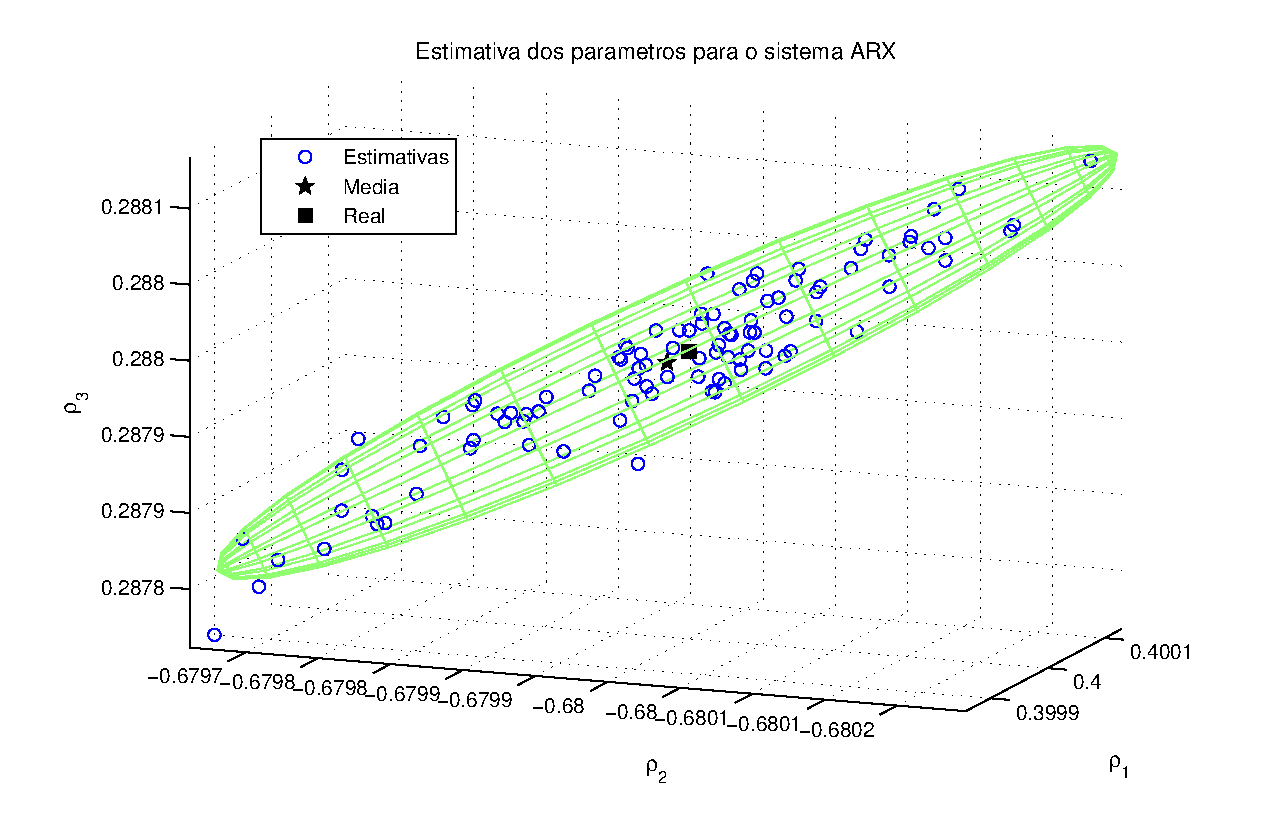
\includegraphics[width=0.95\columnwidth]{figures/vrft_arx_M10_var005_.eps}
	\caption{100 estimativas Monte Carlo dos par�metros $\theta_1$, $\theta_2$ e $\theta_3$ para o controlador
	apresentado em \eqref{eq:vrft_methos_ex_arx_c} com vari�ncia do ru�do $\sigma_e ^2=0.005$}
	\label{fig:vrft_arx_M10_var005}
\end{figure}

Como j� foi observado a utiliza��o de vari�veis instrumentais melhora significativamente o erro de polariza��o existente
nas estimativas do m�todo VRFT quaando h� presen�a de ru�do. Desta forma as informa��es apresentadas a seguir ser�o
feitas utilizando vari�veis instrumentais. Na figura (\ref{fig:vrft_arx_M10_var05_iv}) � apresentado a estimativa dos
par�metros do controlador para um ru�do de vari�ncia $\sigma_e ^2=0.05$. Observa-se que n�o h� erro de polariza��o nas
estimativas. O custo para esta, e outas, estimativas � apresentado na Tabela (\ref{table:vrft_method_arx_iv}).

\begin{figure}[htbp] 
	\center 
	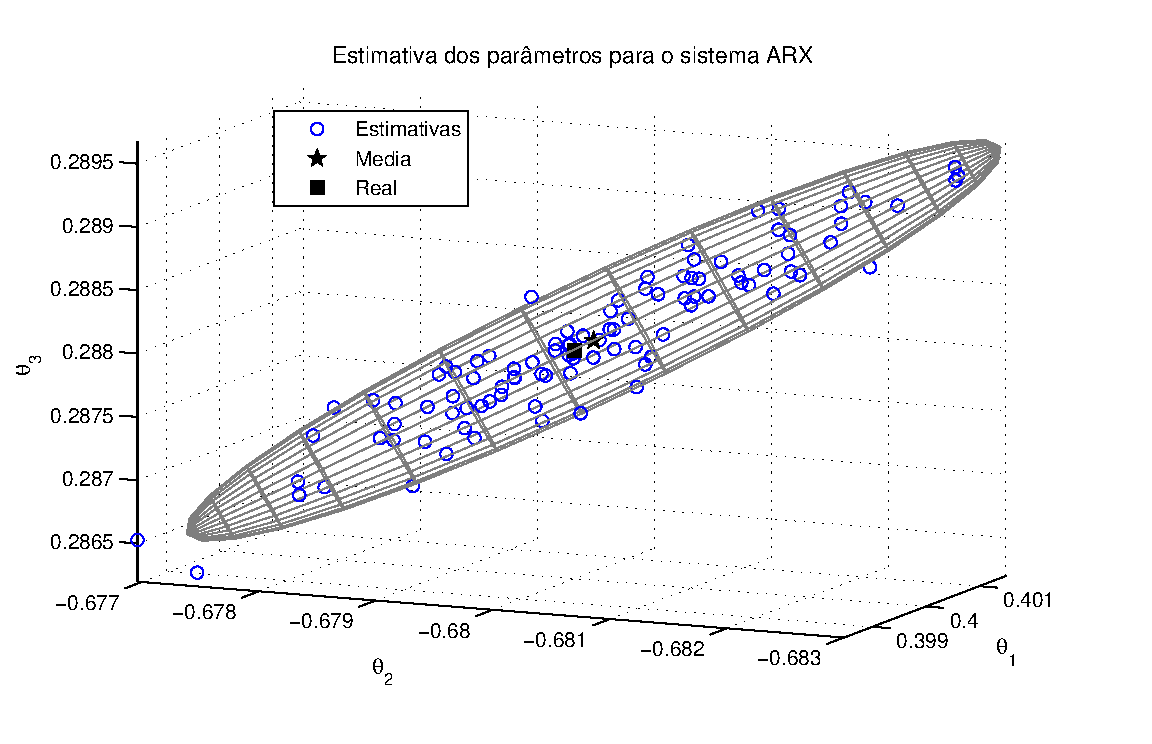
\includegraphics[width=0.95\columnwidth]{figures/vrft_arx_M10_var05_iv.eps}
	\caption{100 estimativas Monte Carlo dos par�metros $\theta_1$, $\theta_2$ e $\theta_3$ para o controlador
	apresentado em \eqref{eq:vrft_methos_ex_arx_c} com vari�ncia do ru�do $\sigma_e ^2=0.05$ utilizando
	vari�veis instrumentais}
	\label{fig:vrft_arx_M10_var05_iv}
\end{figure}


\begin{table*}[htbp]
\begin{center}
\caption{Valor dos custos $J_{VR}^N$ e $J_{y}$ al�m da  vari�ncia das
estimativas para diferentes valores de $\sigma_e^2$ quando o m�todo
VRFT utiliza vari�veis instrumentais para a estimativa dos par�metros $\theta$ do controlador
\eqref{eq:vrft_methos_ex_arx_c}}
\label{table:vrft_method_arx_iv}
\begin{tabular}{cccc}
\hline
        Vari�ncia $\sigma_e^2$ & $J_{VR}^N(\theta)$ &
        $J_{y}(\theta)$ & Vari�ncia estimativas $\theta$   \\
\hline
   0.1     & $10.0743\times10^{-3}$ &  2.2871$\times10^{-3}$ & $1\times10^{-5}\;[0.1253 \; 0.4683 \; 0.1600]$ \\
   0.06    & $ 3.6093\times10^{-3}$ &  1.1279$\times10^{-3}$ & $1\times10^{-5}\;[0.0516 \; 0.1793 \; 0.0575]$ \\
   0.05    & $ 2.5419\times10^{-3}$ &  1.2453$\times10^{-3}$ & $1\times10^{-5}\;[0.0344 \; 0.1237 \; 0.0416]$ \\
   0.04    & $ 1.6013\times10^{-3}$ &  0.5106$\times10^{-3}$ & $1\times10^{-6}\;[0.2195 \; 0.7908 \; 0.2379]$ \\
   0.01    & $10.0077\times10^{-5}$ & 13.7142$\times10^{-5}$ & $1\times10^{-7}\;[0.1552 \; 0.5469 \; 0.1822]$ \\
   0.005   & $ 2.5081\times10^{-5}$ & 10.3482$\times10^{-5}$ & $1\times10^{-7}\;[0.0406 \; 0.1260 \; 0.0375]$ \\
	0.001  & $ 0.1009\times10^{-5}$ &  2.0487$\times10^{-5}$ & $1\times10^{-9}\;[0.1277 \; 0.4035 \;0.1239]$	 \\
\hline
\end{tabular}
\end{center}
\end{table*}

%===============================================================================
\subsubsection{Controlador n�o pertence a classe}
\label{sec:dbcd_vrft_examples_not_in_class}
%===============================================================================

At� este ponto foram apresentados exemplos de uso do m�todo VRFT quando o controlador que leva o sistema para
o comportamento desejado $T_d(z)$ faz parte da classe escolhida para a identifica��o. Nesta se��o ser� apresentado um
exemplo onde a classe de modelos do controlador escolhida n�o consegue represetar o controlador ideal $C_d(z)$.

Considerando o sistema real descrito por:

\begin{equation}
G_{ 0 }(z)=\frac { 0.2(z-0.7) }{ (z-0.9)(z-0.5) } ,\quad \quad \quad H_{ 0 }(z)=\frac { z }{ z-0.3 } 
\nonumber
\end{equation}

Deseja-se que em malha fechada ele se comporte como em: 

\begin{equation}
T_d(z)=\frac { 0.16z }{ (z-0.6)^2 }
\label{eq:vrft_methos_ex_pid_not_M}
\end{equation}

Neste caso o controlador ideal � definido por

\begin{equation}
C_{ d }(z)=\frac { 0.8z(z-0.9)(z-0.5) }{ (z-1)(z-0.36)(z-0.7) } 
\label{eq:vrft_methos_ex_pid_not_cd}
\end{equation}

Para esta identifica��o optou-se por um controlador do tipo PID como em:
 
\begin{equation}
C(z,\theta )=\frac { \theta _{ 1 }z^2+\theta _{ 2 }z+\theta _{ 3 } }{ z(z-1) } 
\label{eq:vrft_methos_ex_pid_not_c}
\end{equation}

Observa-se que \eqref{eq:vrft_methos_ex_pid_not_c} n�o consegue representar todas as din�micas apresentadas em
\eqref{eq:vrft_methos_ex_pid_not_cd}. Utilizando o procedimento descrito na Se��o
(\ref{sec:dbcd_vrft_framework_noise}) e o procedimento de experimento repetido, foram feitos 100 experimentos de
Monte Carlo e o resultado obtido para a m�dia das estimativas foi:

\begin{equation}
\theta_L =\left[ 0.8101 \quad -0.1691  \quad -0.3358 \right]
\nonumber
\end{equation}

onde o �ndice $L$ indica que este resultado foi obtido utilizando-se o filtro $L$.

Repetindo a simula��o, mas agora sem que o procedimento da utiliza��o do filtro $L$ descrito na se��o
(\ref{sec:dbcd_vrft_framework_noise}), obteve-se o resultado seguinte:

\begin{equation}
\theta =\left[ 0.5846 \quad -0.2108  \quad -0.1525 \right]
\nonumber
\end{equation}

Aplicando-se estes resultados ao controlador apresentado em \eqref{eq:vrft_methos_ex_pid_not_c} e de posse do
comportamento desejado para o sistema em malha fechada ($T_d(z)$) � poss�vel fazer um comparativo da resposta
ao salto unit�rio para o sistema utilizando os dois controladores obtidos. O resultado � apresentado na Figura
(\ref{fig:vrft_notinclass_step}).

\begin{figure}[htbp] 
	\center 
	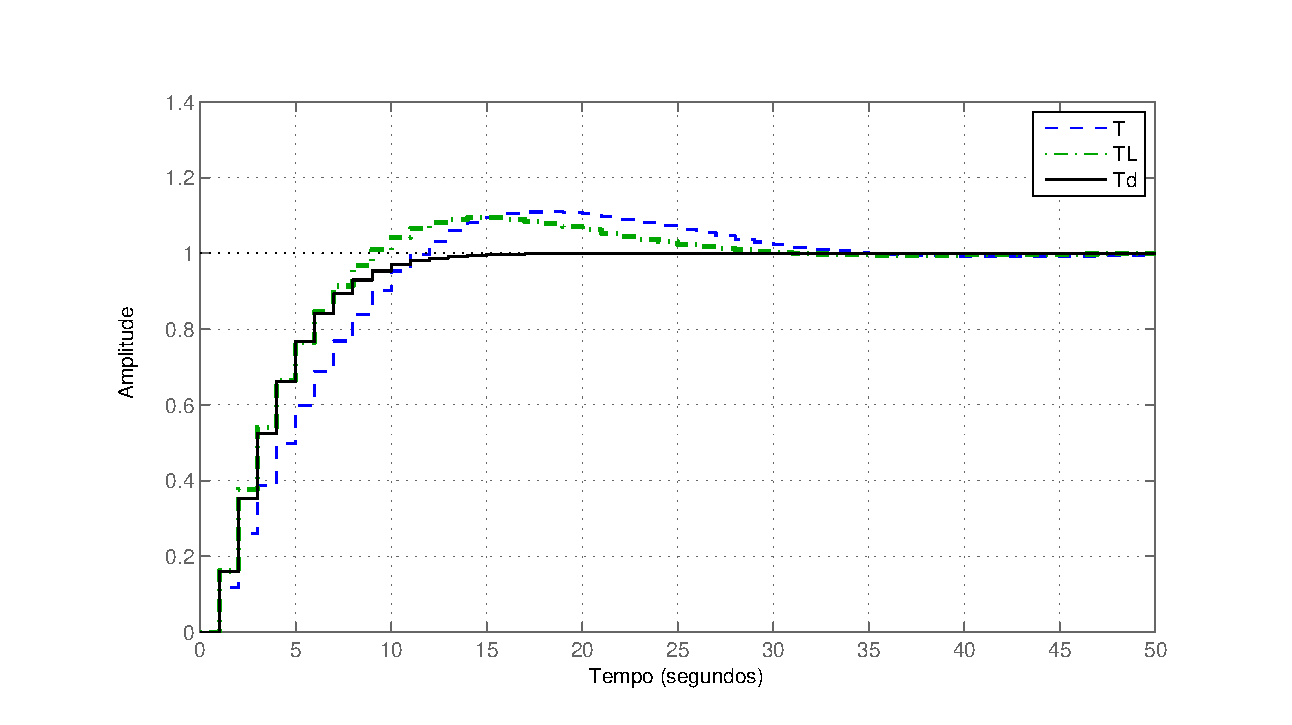
\includegraphics[width=0.85\columnwidth]{figures/vrft_notinclass_step.eps}
	\caption{Comparativo da resposta do sistema a um degrau unit�rio quando o controlador inserido � obtido pelo
	m�todo VRFT utilizando o filtro L e quando n�o se utiliza este artificio. O sistema foi simulado com um
	ru�do de vari�ncia $\sigma_e ^2=0.1$}
	\label{fig:vrft_notinclass_step}
\end{figure}

Observa-se que para o sistema que utiliza o controlador estimado utilizando-se o filtro $L$, a resposta ao
degrau unit�rio tem significativamente menos erro que o sistema utilizando o outro controlador. Ficando este
primeiro muito mais pr�ximo da fun��o $T_d(z)$ desejada.

Os custos destes dois sistemas � apresentado na Tabela (\ref{table:vrft_method_notinclass}).

\begin{table*}[htbp]
\begin{center}
\caption{Valor dos custos $J_{VR}^N$ e $J_{y}$ para o sistema controlado por $C(z)$ e $C_L(z)$}
\label{table:vrft_method_notinclass}
\begin{tabular}{ccc}
\hline
        Controlador & $J_{VR}^N(\theta)$ & $J_{y}(\theta)$ \\
\hline
	$C(z)$   & 0.2877 &  0.1270 \\
	$C_L(z)$ & 0.4481 &  0.0542 \\
\hline
\end{tabular}
\end{center}
\end{table*}

A fim de comparar as duas estimativas, na figura (\ref{fig:vrft_notinclass_bode}) � apresentado o diagrama de
Bode dos controladores obtidos (utilizando a m�dia das estimativas obtidas).

\begin{figure}[htbp] 
	\center 
	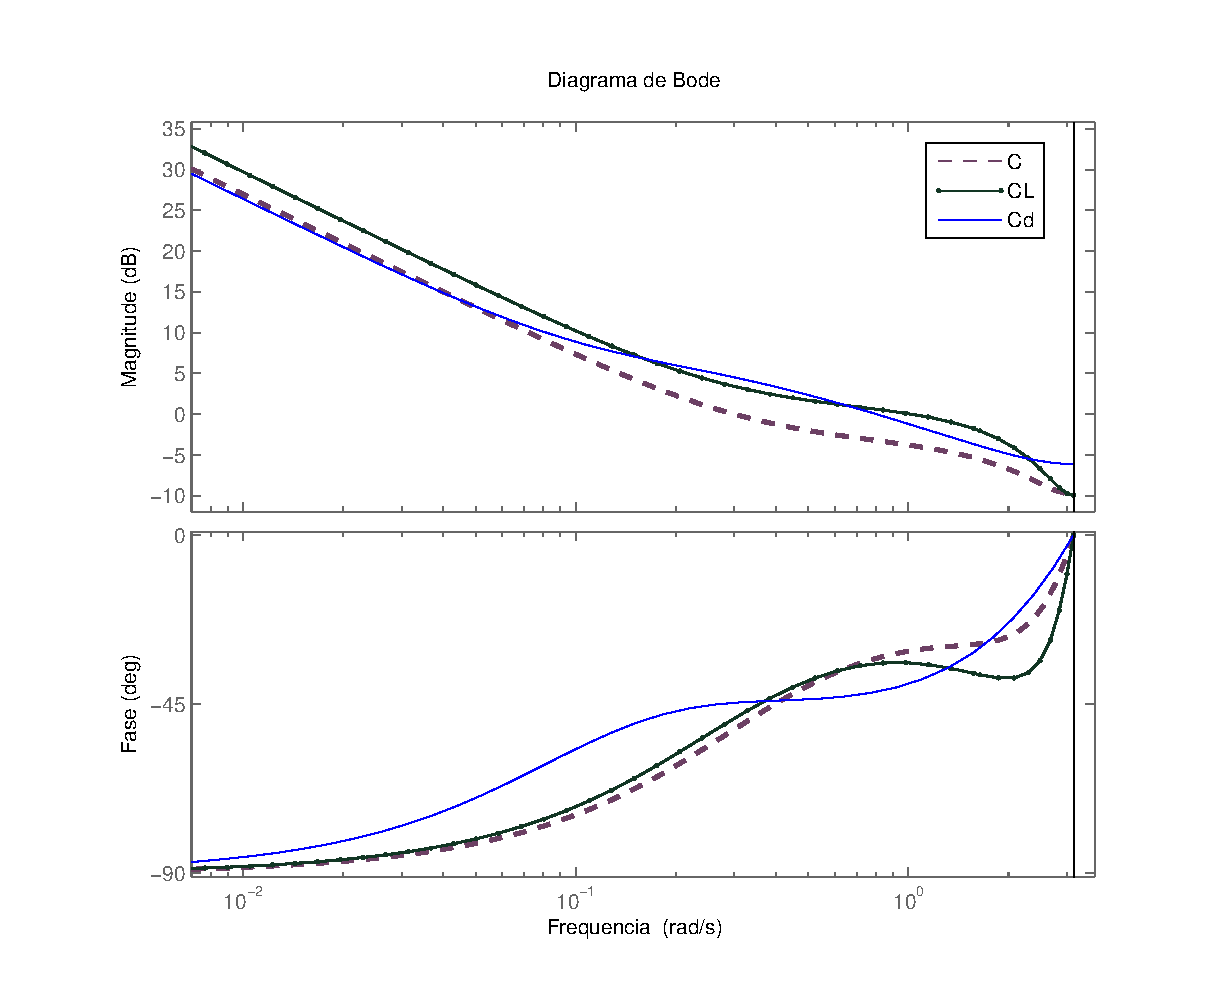
\includegraphics[width=0.85\columnwidth]{figures/vrft_notinclass_bode.eps}
	\caption{Diagrama de Bode para as fun��es de transfer�ncia dos controladores estimados utilizando VRFT com e
	sem o artificio do filtro L e vari�veis instrumentais}
	\label{fig:vrft_notinclass_bode}
\end{figure}


%===============================================================================
\chapter{Identifica��o de sistemas n�o lineares}
\label{chapter:non_linear_sis_ident}
%===============================================================================

%===============================================================================
%===============================================================================
\section{Lineariza��o de sistemas}
\label{sec:non_linear_si_linearization}
%===============================================================================


%===============================================================================
\section{Modelos para sistemas n�o lineares}
\label{sec:nl_models}
%===============================================================================

\cite{CampiSacvaresi-vrft_nonlinear}

%===============================================================================
\subsection{Modelos de Wiener e Hammerstein}
\label{sec:nl_models_wiener_hammerstein}
% Aguirre: 334
% ljung 143
%===============================================================================


%===============================================================================
\subsection{Serie de volterra}
\label{sec:nl_models_volterra}
% Aguirre 334
%===============================================================================


%===============================================================================
\subsection{Fun��es Radiais de Base}
\label{sec:nl_models_radiais}
% Aguirre 337
%===============================================================================



%===============================================================================
\subsection{Modelo polinomial NARMAX}
\label{sec:nl_models_pol_narmax}
% Aguirre 343
%===============================================================================


%===============================================================================
\subsection{Modelo Racional NARMAX}
\label{sec:nl_models_rational_narmax}
% Aguirre 343
%===============================================================================

%===============================================================================
\section{Algoritmos para identifica��o}
\label{sec:non_linear_si_algorithms}
%===============================================================================

%===============================================================================
\subsection{Modelos Racionais}
\label{sec:nl_algorithms_rationals}
% Aguirre 393
% Tese do corr�a - pg 27
%===============================================================================

\input{tex/chapters/non_linear_si_conclusions}
%===============================================================================


% \chapter{Estado da arte}
% \chapter{Mais estado da arte}
% \chapter{A minha contribui��o}
% \chapter{Prova de que a minha contribui��o � v�lida}
% \chapter{Conclus�o}

% referencias
% Aqui pode ser usado o ambiente padrao `thebibliography'; por�m, fa�a um
% favor a s� mesmo e use o \bibtex\ e o estilo abnt.bst (veja na p�gina do
% UTUG). 

\bibliographystyle{abnt}

%\bibliography{exemplo,modelo} 	% pode-se ter v�rios arquivos .bib separados
\bibliography{disssertacao_neuhaus} 	% pode-se ter v�rios arquivos .bib separados
				% por v�rgulas. Segundo a NBR6023, as
				% refer�ncias devem ser alinhadas apenas a
				% esquerda. � esquisito, mas � assim.

% Ap�ndices
\appendix

% Pode-se ter diversos ap�ndices
\chapter{T�tulo do Ap�ndice}

Nos ap�ndices aparecem textos ou documentos elaborados pelo autor  a fim de
complementar sua argumenta��o sem preju�zo do trabalho. Eles sempre dever�o
estar depois das refer�ncias e antes dos anexos.


% Anexos
\annex

% Pode-se ter diversos anexos
\chapter{T�tulo do Anexo}

J� os anexos ser�o textos, trabalhos e materiais que n�o foram elaborados
pelo autor, mas que servem de comprova��o, fundamenta��o ou ilustra��o dos
argumentos contidos no texto. Neste ponto, deve-se dar especial aten��o �
quest�o dos direitos autorais.

\end{document}
